\documentclass[preprint,12pt]{elsarticle}
\usepackage[T1]{fontenc}
\usepackage{lmodern}
\usepackage{amsmath,amssymb,amsfonts,amsthm,mathtools}
\usepackage{booktabs,multirow,array,tabularx}
\usepackage{graphicx}
\usepackage{float}
\usepackage{xcolor}
\usepackage{tikz}
\usepackage{etoolbox}
\usepackage[hidelinks]{hyperref}
\usepackage{url}
\usepackage{microtype}
\usepackage{enumitem}
\usepackage{siunitx}
\usepackage{placeins}
\usepackage{flafter}
\setlength{\textfloatsep}{14pt plus 2pt minus 4pt}
\setlength{\floatsep}{10pt plus 2pt minus 3pt}
\usetikzlibrary{arrows,positioning}
\newfloat{algorithm}{tbp}{loa}
\floatname{algorithm}{Algorithm}
\floatstyle{ruled}
\restylefloat{algorithm}
\allowdisplaybreaks
\graphicspath{{figures/}}
\journal{Pattern Recognition}
\date{Oct. 28, 2026}
\biboptions{numbers,sort&compress}
\newtheorem{theorem}{Theorem}
\newtheorem{proposition}{Proposition}
\newtheorem{lemma}{Lemma}
\newtheorem{corollary}{Corollary}
\theoremstyle{remark}
\newtheorem{remark}{Remark}
\newcommand{\R}{\mathbb{R}}
\newcommand{\one}{\mathbf{1}}
\newcommand{\diag}{\operatorname{diag}}
\providecommand{\doi}[1]{\href{https://doi.org/#1}{doi:#1}}
\DeclareMathOperator*{\argmax}{arg\,max}

\begin{document}
\raggedbottom
\begin{frontmatter}
\title{Scale--Semantic Separated Nonnegative Matrix Factorization for Semi-Supervised Clustering}
\author{Deshu Sun}
\author{Feng Wang\corref{cor1}}
\cortext[cor1]{Corresponding author}
\ead{wangfeng@gzmu.edu.cn}
\address{College of Data Science and Information Engineering, Guizhou Minzu University, Guiyang, Guizhou 550025, P.R. China}
\begin{abstract}
Semi-supervised nonnegative matrix factorization (NMF) often uses one latent coefficient both to reconstruct a sample and to represent its class. Clamping a labeled coefficient to a one-hot vector fixes its semantic direction and reconstruction amplitude. We propose scale-semantic separated NMF (ScaleSem-NMF), which writes each coefficient as a nonnegative scalar amplitude multiplied by a simplex-valued semantic direction. Labels and graph propagation act on the semantic direction, while reconstruction learns the amplitude. The objective contains a reconstruction term and a positive-semidefinite high-order diffusion term. We derive a multiplicative basis update, an exact nonnegative amplitude update, and an Armijo projected-gradient semantic update. Eight-dataset experiments with 20 paired seeds show the strongest dual-metric gains on COIL20 and COIL100, positive paired effects on AR and MNIST relative to HLPNMF, and practical parity on Optdigits, PIE, and MSRA25. A 1600-run supervision-budget experiment passes the preregistered low-label gate. Under salt-and-pepper corruption, ScaleSem-NMF stays within 0.01 ACC and NMI of the strongest baseline on COIL20, PIE, and YaleB at every tested level through 30\%. Runtime and parameter analyses quantify computational cost and neighborhood sensitivity. These results support scale-semantic separation as an interpretable structural alternative for semi-supervised NMF.
\end{abstract}
\begin{keyword}
semi-supervised clustering \sep nonnegative matrix factorization \sep scale-semantic separation \sep label propagation \sep simplex representation
\end{keyword}
\end{frontmatter}

\section{Introduction}

Clustering and semi-supervised learning use structural assumptions and limited annotation to reduce the ambiguity of an otherwise unsupervised partition \cite{Jain1999Clustering,Jain2010Clustering,VanEngelen2020Survey,Bair2013SSC}. Nonnegative matrix factorization (NMF) is attractive in this setting because its additive latent coefficients can be interpreted as class evidence \cite{Lee1999NMF,Lee2001Algorithms,Gillis2014WhyHow}. Existing semi-supervised NMF methods impose label constraints, discriminative penalties, graph or hypergraph regularization, and label propagation on those coefficients \cite{Liu2012CNMF,Xing2021DSSNMF,Li2025EDNMF,Shen2026LCNMF,Cai2011GNMF,Zeng2014HypergraphNMF,Yi2015LpSNMF,Lan2022LPNMF,Wang2022PNLP}.

Compact label-guided NMF models frequently use the same coefficient vector for two roles. In the reconstruction model, its magnitude controls sample amplitude. In the supervision model, a one-hot vector represents normalized class semantics. Directly setting a labeled coefficient equal to its one-hot label therefore fixes both its direction and its radial magnitude. Input normalization does not remove this issue because the amplitude required in a learned nonnegative basis remains sample and basis dependent.

Direct and propagation-guided models provide the closest context. GOCNMF and OCSNMF impose one-hot semantics directly in graph or symmetric factorizations \cite{Li2025GOCNMF,Li2025OCSNMF}; constraint propagation, hypergraph propagation, pivotal-aware propagation, and joint label/constraint propagation transfer supervision through different relational objects \cite{Wang2015ConstraintNMF,Yin2023HSSNMF,Yang2025SPNMF,Mo2024PNLPSCNMF}. Robust semi-supervised NMF further changes the reconstruction loss \cite{Peng2021CSNMF}, whereas magnitude-aware supervision explicitly questions the information discarded by binary labels \cite{Jing2025SNMFSP}. SNMFWLP and HLPNMF couple reconstruction with weighted or high-order propagation through learned representations \cite{Jing2026SNMFWLP,Li2026HLPNMF}. These methods motivate a precise question: can reconstruction amplitude and class semantics be represented separately while preserving a compact, directly decodable NMF model?

ScaleSem-NMF answers this question by writing every coefficient as

\[
v_i=s_i f_i,\qquad s_i\ge 0,\quad f_i\ge 0,\quad \mathbf 1_c^\top f_i=1.
\]

The scalar \(s_i\) is reconstruction driven, whereas \(f_i\) is a semantic direction. Only \(f_i\) is clamped to a known label and smoothed over the graph. Its relation to magnitude-aware supervision and simplex-structured factorization is discussed in Section~2; the distinguishing operation is to learn sample amplitudes jointly while excluding them from graph propagation.

The contributions are fourfold.

\begin{enumerate}
\item We identify point anchoring as a structural coupling between semantic direction and reconstruction amplitude and replace it with a sample-wise scale-semantic decomposition.
\item We formulate a compact ScaleSem-NMF objective with a simplex semantic matrix and a symmetric positive-semidefinite high-order graph operator.
\item We give block updates with an exact amplitude step and feasibility-preserving semantic descent, together with explicit assumptions for monotonicity and conditional stationarity.
\item We evaluate the model under protocols fixed before formal analysis. The evidence includes eight-dataset paired comparisons, five supervision budgets, parameter sensitivity, controlled ablations, salt-and-pepper corruption, convergence, unified single-thread timing, and nested PIE resource measurements.
\end{enumerate}

\section{Related work}

\subsection{Semi-supervised NMF}

Standard NMF approximates \(X\in\mathbb R_+^{d\times n}\) by \(UV^\top\), where \(U\in\mathbb R_+^{d\times c}\) is a basis and \(V\in\mathbb R_+^{n\times c}\) contains sample coefficients. Semi-supervised variants constrain \(V\), learn a label mapping, encode pairwise relations, or regularize a sample graph \cite{Liu2012CNMF,Xing2021DSSNMF,Cai2011GNMF,Yi2015LpSNMF}. ScaleSem-NMF belongs to the direct-decoding family: class prediction uses the largest semantic coordinate and does not add a separate classifier.

S4NMF derives self-supervision from the consensus of ensembled NMF solutions and feeds similarity and dissimilarity information back into factorization \cite{Chavoshinejad2023S4NMF}. ScaleSem-NMF addresses the coefficient geometry of direct label anchoring through a sample-wise amplitude and semantic direction.

\subsection{Label propagation and high-order diffusion}

Let \(A=A^\top\ge0\) be a symmetric sample affinity matrix and \(D=\operatorname{diag}(A\mathbf 1_n)\), with strictly positive degrees. The normalized symmetric operator is

\[
P=D^{-1/2}AD^{-1/2}.
\]

Graph label propagation assumes that nearby samples have similar semantic representations \cite{Zhu2003GaussianFields,Zhou2004LGC}. Graph construction quality and propagation bias are consequently material modeling choices \cite{Qiao2018GraphReview,Gao2022HypergraphReview,Song2023GSSLReview}. HLPNMF uses multi-step propagation inside NMF \cite{Li2026HLPNMF}. ScaleSem-NMF retains propagation depth but applies it only to the normalized semantic direction.

\subsection{Magnitude-aware and simplex representations}

Magnitude-aware supervision observes that binary labels may discard useful sample scale \cite{Jing2025SNMFSP}. Simplex factorizations interpret normalized coefficients as soft memberships \cite{Abdolali2021SSMF}, while dual-simplex formulations use polytope polarity to control identifiability and volume \cite{Abdolali2024DualSimplex}. Discriminative graph NMF provides a related example of coupling neighborhood structure with label separation \cite{Xing2021GNMFLD}. These ideas do not by themselves resolve partially labeled graph propagation. ScaleSem-NMF combines a learned radial amplitude with a simplex semantic direction, so that reconstruction and supervision act on different variables.

\section{Methodology}

\subsection{Point anchoring and scale-semantic decomposition}

For labeled sample \(i\), direct coefficient anchoring imposes \(v_i=y_i\), where \(y_i\) is one-hot. Under \(x_i\approx Uv_i^\top\), this forces \(x_i\approx Uy_i^\top\): every labeled sample in a class is assigned the same unit latent amplitude. ScaleSem-NMF instead defines

\[
v_i=s_i f_i,\qquad f_i\in\Delta^{c-1}
=\{f\in\mathbb R_+^c:\mathbf 1_c^\top f=1\}.
\]

With \(F=[f_1^\top;\ldots;f_n^\top]\in\mathbb R_+^{n\times c}\) and \(s\in\mathbb R_+^n\),

\[
V=\operatorname{diag}(s)F.
\]

For any nonzero \(v_i\), the decomposition is uniquely fixed by \(s_i=\lVert v_i\rVert_1\) and \(f_i=v_i/s_i\). A global gauge between \(U\) and \(s\) remains and is normalized numerically.

This decomposition alone is a row-wise reparameterization of a nonnegative coefficient matrix. Indeed, if every row of \(V\ge0\) has positive sum and \(r=V\mathbf 1_c\), then
\begin{equation}
\label{eq:row_normalized_semantics}
s=r,\qquad F=\diag(r)^{-1}V,qquad V=\diag(s)F.
\end{equation}
Consequently, the reconstruction term is unchanged. The substantive modeling choice is that labels and high-order diffusion act on the row-normalized semantic directions \(F\), rather than on the amplitude-bearing coefficients \(V\). Equivalently, over positive-row \(V\), the regularizer is
\begin{equation}
\label{eq:direction_regularizer}
\alpha\operatorname{Tr}\!\left[
\bigl(\diag(V\mathbf 1_c)^{-1}V\bigr)^\top L_k
\bigl(\diag(V\mathbf 1_c)^{-1}V\bigr)
\right].
\end{equation}
If \(s_i=0\), reconstruction is independent of \(f_i\); its semantic direction remains constrained by the simplex, the labeled rows, and graph diffusion. The stationarity result below therefore states explicit nondegeneracy conditions for the reconstruction blocks.

\subsection{Objective and graph operator}

Figure~\ref{fig:overview} summarizes the role-specific coupling. Its upper branch constructs the positive-semidefinite high-order diffusion operator from sample geometry; its lower branch decomposes each coefficient into reconstruction amplitude \(s_i\) and simplex semantic direction \(f_i\). Reconstruction uses \(U,s,F\), whereas partial labels and diffusion constrain only \(F\). Prediction is therefore decoded directly from \(F\), without letting sample amplitude enter label propagation.

\begin{figure*}[t]
\centering
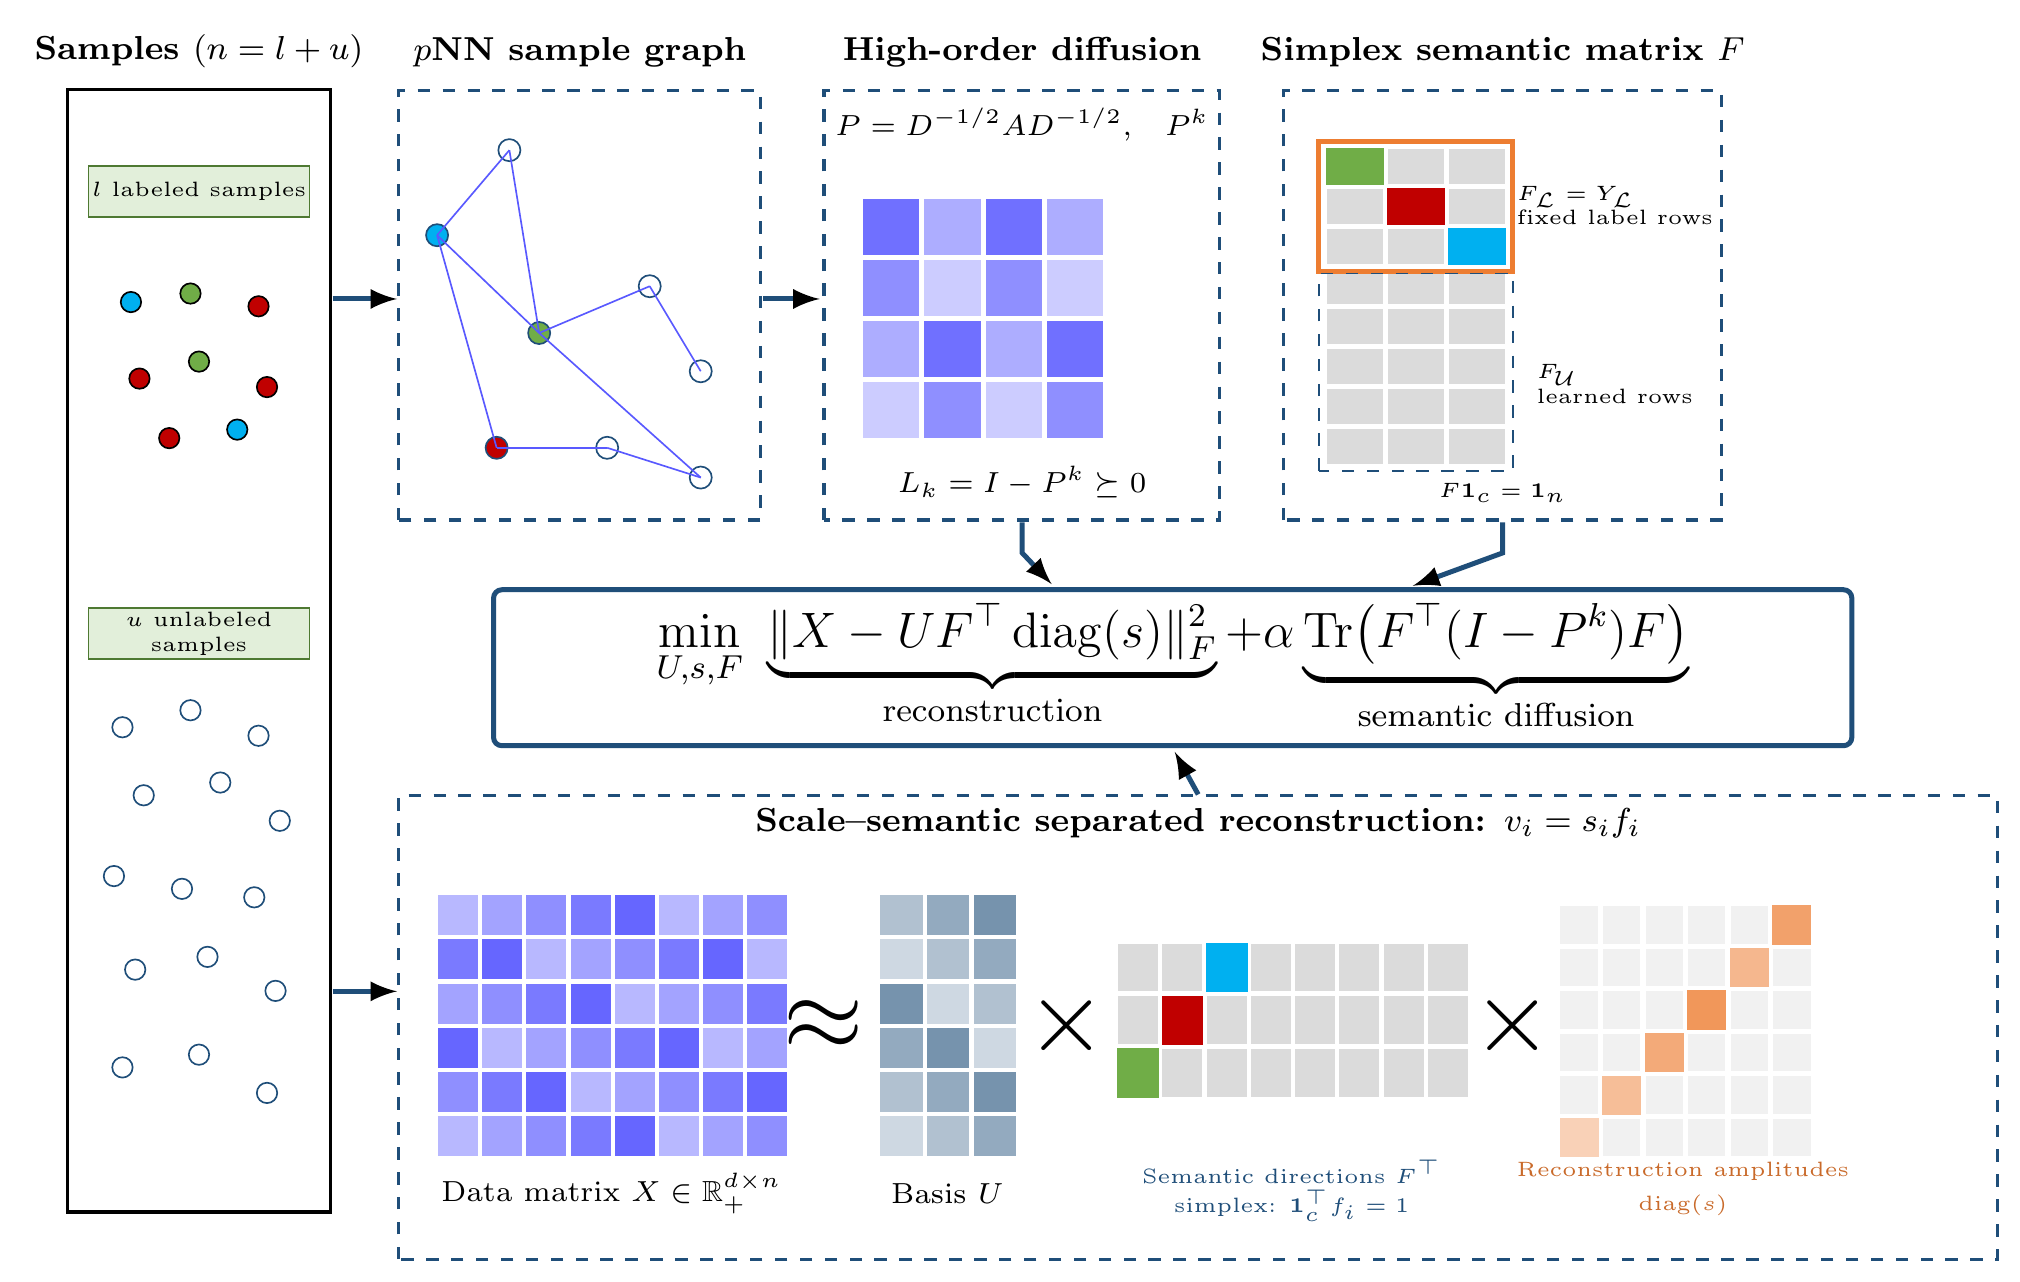
\includegraphics[width=0.90\textwidth,height=0.66\textheight,keepaspectratio]{figures/png/method-overview.png}
\caption{Mechanism of ScaleSem-NMF. The geometry branch produces the high-order operator \(L_k\), while the factorization branch separates coefficient amplitude from semantic direction. The two branches meet in one objective, but labels and diffusion act only on the simplex semantic matrix \(F\).}
\label{fig:overview}
\end{figure*}

All experiments use an affinity induced by a weighted neighborhood hypergraph. For samples \(x_i\), define the Gaussian similarities
\begin{equation}
\label{eq:gaussian_affinity}
K_{ij}=\exp\!\left(-\frac{\lVert x_i-x_j\rVert_2^2}{\sigma^2}\right),
\qquad
\sigma=\frac{1}{n^2}\sum_{i=1}^n\sum_{j=1}^n\lVert x_i-x_j\rVert_2.
\end{equation}
The hyperedge \(e_i\) contains center sample \(i\) and its \(p\) nearest neighbors. With \(m=n\) hyperedges, let \(H\in\{0,1\}^{m\times n}\) satisfy \(H_{ij}=1\) if sample \(j\in e_i\), and define
\begin{equation}
\label{eq:hypergraph_affinity}
\begin{aligned}
w_i&=\sum_{j\in e_i}K_{ij},&
W&=\diag(w_1,\ldots,w_m),\\
D_e&=\diag(H\mathbf 1_n),&
\Theta&=H^\top W D_e^{-1}H.
\end{aligned}
\end{equation}
The implementation then uses
\begin{equation}
\label{eq:symmetric_operator}
A=\frac{\Theta+\Theta^\top}{2},\qquad
D=\diag(A\mathbf 1_n),\qquad
P=D^{-1/2}AD^{-1/2}.
\end{equation}
Thus the hypergraph is used to construct a symmetric nonnegative sample affinity; the optimized variables remain \(U,s,F\). For an integer \(k\ge1\), define

\[
L_k=I_n-P^k.
\]

\textbf{Proposition 1.} If \(A\) is symmetric, nonnegative, and has positive degrees, then \(L_k\succeq0\) for every positive integer \(k\).

\textbf{Proof.} The matrix \(P\) is symmetric and
\[
P=D^{1/2}(D^{-1}A)D^{-1/2},
\]
so it is similar to the row-stochastic matrix \(D^{-1}A\). Hence the eigenvalues of \(P\) are real and belong to \([-1,1]\). If \(\lambda_i(P)\) is an eigenvalue of \(P\), the corresponding eigenvalue of \(L_k\) is \(1-\lambda_i(P)^k\ge0\) for every positive integer \(k\). Thus \(L_k\succeq0\). \(\square\)

Let \(\mathcal L\) be the labeled index set and \(Y_{\mathcal L}\) the one-hot labels. ScaleSem-NMF solves

\begin{equation}
\label{eq:scalesemnmf_objective}
\begin{aligned}
\min_{U,s,F}\quad &
J(U,s,F)=\left\lVert X-UF^\top\operatorname{diag}(s)\right\rVert_F^2
+\alpha\operatorname{Tr}(F^\top L_kF),\\
\text{s.t.}\quad &U\ge0,\quad s\ge0,\quad F\ge0,\\
&F\mathbf 1_c=\mathbf 1_n,\quad F_{\mathcal L}=Y_{\mathcal L}.
\end{aligned}
\end{equation}

Prediction is direct: \(\widehat y_i=\arg\max_q F_{iq}\).

\subsection{Block optimization}

With \(V^t=\operatorname{diag}(s^t)F^t\), the basis update is

\begin{equation}
\label{eq:update_u}
\widetilde U^{t+1}=U^t\odot
\frac{XV^t}{U^t((V^t)^\top V^t)}.
\end{equation}

The implementation uses a machine-scale denominator safeguard only when needed. A fixed additive \(\varepsilon>0\) changes the fixed-point equation and therefore cannot be used in a stationarity proof for the unperturbed objective. Theorem 2 consequently assumes that the safeguard is eventually inactive (or that a vanishing safeguard is used).

For fixed \(\widetilde U^{t+1},F^t\), set \(g_i^{t+1}=\widetilde U^{t+1}(f_i^t)^\top\). Each amplitude has the exact update

\begin{equation}
\label{eq:update_s}
\widetilde s_i^{t+1}=
\begin{cases}
\max\!\left(0,\dfrac{(g_i^{t+1})^\top x_i}{(g_i^{t+1})^\top g_i^{t+1}}\right),&g_i^{t+1}\ne0,\\
0,&g_i^{t+1}=0.
\end{cases}
\end{equation}

The global gauge is normalized by
\begin{equation}
\label{eq:update_gauge}
\beta^{t+1}=\lVert\widetilde U^{t+1}\rVert_F,qquad
U^{t+1}=\frac{\widetilde U^{t+1}}{\beta^{t+1}},qquad
s^{t+1}=\beta^{t+1}\widetilde s^{t+1},
\end{equation}
which leaves the reconstruction unchanged. Here tildes denote the basis and amplitude after their block updates but before gauge normalization.

Let \(D_s=\operatorname{diag}(s)\). The semantic gradient is

\begin{equation}
\label{eq:gradient_f}
\nabla_FJ=2D_s^2F(U^\top U)-2D_sX^\top U+2\alpha L_kF.
\end{equation}

For a backtracking step size \(\eta_t>0\), the semantic update is
\begin{equation}
\label{eq:update_f}
F^{t+1}=\Pi_{\mathcal C}\!\left(F^t-\eta_t\nabla_FJ(U^{t+1},s^{t+1},F^t)\right),
\end{equation}
where \(\mathcal C\) enforces unlabeled simplex rows and fixed labeled rows. Backtracking accepts the candidate \(\widehat F\) when

\begin{equation}
\label{eq:armijo}
J(U,s,\widehat F)\le J(U,s,F)
+\sigma\langle\nabla_FJ,\widehat F-F\rangle,
\qquad 0<\sigma<1.
\end{equation}

For completeness, let \(z\in\mathbb R^c\) and write its sorted entries as \(z_{(1)}\ge\cdots\ge z_{(c)}\). Define
\begin{equation}
\label{eq:simplex_projection}
q=\max\left\{j:\ z_{(j)}-\frac{\sum_{\ell=1}^{j}z_{(\ell)}-1}{j}>0\right\},\qquad
\tau=\frac{\sum_{\ell=1}^{q}z_{(\ell)}-1}{q}.
\end{equation}
The Euclidean simplex projection is \([\Pi_{\Delta^{c-1}}(z)]_j=\max\{z_j-\tau,0\}\). Accordingly, \(\Pi_{\mathcal C}\) applies this projection row-wise to unlabeled samples and restores every labeled row to \(Y_{\mathcal L}\). This operation costs \(O(nc\log c)\) with sorting.

\subsection{Algorithm}

The complete optimization procedure is summarized in Algorithm~\ref{alg:scalesemnmf}. Its order is important: the amplitude is minimized after the basis update, gauge normalization is applied before semantic descent, and the stopping test is evaluated only after a complete block cycle.

\begin{algorithm}[H]
\caption{Optimization procedure for ScaleSem-NMF}
\label{alg:scalesemnmf}
\scriptsize
\textbf{Input:} Data matrix \(X\in\mathbb R_+^{d\times n}\); labeled index set \(\mathcal L\) and one-hot label matrix \(Y_{\mathcal L}\); number of classes \(c\); neighborhood size \(p\); propagation order \(k\); regularization parameter \(\alpha\); maximum iterations \(T\); tolerance \(\varepsilon\); Armijo parameters \(\eta_0,\rho,\sigma\).\\
\textbf{Output:} Basis \(U\), amplitudes \(s\), semantic matrix \(F\), and predicted labels \(\widehat y\).

\textbf{Precomputation:}
\begin{enumerate}[label=\arabic*.,leftmargin=5mm,itemsep=1pt,topsep=1pt]
\item Normalize each sample to unit \(\ell_2\) norm. Construct \(K,H,W,D_e,\Theta,A,D,P\) using \eqref{eq:gaussian_affinity}--\eqref{eq:symmetric_operator}, and set \(L_k=I-P^k\).
\end{enumerate}
\textbf{Initialization:}
\begin{enumerate}[label=\arabic*.,leftmargin=5mm,itemsep=1pt,topsep=1pt,start=2]
\item Draw \(U_{ij}\) and an auxiliary coefficient matrix \((V_0)_{ij}\) independently from \(\operatorname{Unif}(0,1)\), replace numerical zeros by machine epsilon, set \(s=V_0\mathbf 1_c\) and \(F=\diag(s)^{-1}V_0\), and set \(F_{\mathcal L}=Y_{\mathcal L}\). Re-estimate each labeled amplitude using \eqref{eq:update_s} before the first complete iteration.
\item Evaluate \(J^{(0)}\) from \eqref{eq:scalesemnmf_objective}.
\end{enumerate}
\textbf{Iterative updates:}
\begin{enumerate}[label=\arabic*.,leftmargin=5mm,itemsep=1pt,topsep=1pt,start=4]
\item \textbf{for} \(t=0,\ldots,T-1\) \textbf{do}
\begin{enumerate}[label=\alph*.,leftmargin=5mm,itemsep=1pt,topsep=1pt]
\item Set \(V^t=\operatorname{diag}(s^t)F^t\), and compute \(\widetilde U^{t+1}\) using \eqref{eq:update_u}.
\item For \(i=1,\ldots,n\), set \(g_i^{t+1}=\widetilde U^{t+1}(f_i^t)^\top\) and compute \(\widetilde s_i^{t+1}\) using \eqref{eq:update_s}.
\item Normalize \((\widetilde U^{t+1},\widetilde s^{t+1})\) using \eqref{eq:update_gauge}.
\item Compute \(\nabla_FJ(U^{t+1},s^{t+1},F^t)\) using \eqref{eq:gradient_f}. Starting from \(\eta_t=\eta_0\), reduce \(\eta_t\leftarrow\rho\eta_t\) until the candidate in \eqref{eq:update_f} satisfies \eqref{eq:armijo}, and then accept \(F^{t+1}\).
\item Evaluate \(J^{(t+1)}\). If
\[
\frac{\lvert J^{(t+1)}-J^{(t)}\rvert}{\max\{1,J^{(t)}\}}\le\varepsilon,
\]
\textbf{break}.
\end{enumerate}
\item \textbf{end for}
\end{enumerate}
\textbf{Prediction:} For every unlabeled sample, assign
\(\widehat y_i=\arg\max_{1\le q\le c}F_{iq}\), and return \(U,s,F,\widehat y\).
\end{algorithm}

\subsection{Convergence statement}

\textbf{Theorem 1 (monotonic descent and objective convergence).}
Suppose \(L_k\succeq0\), all multiplicative-update denominators are positive, the denominator safeguard is inactive (or vanishes), and the Armijo search terminates. Then every complete ScaleSem-NMF cycle satisfies
\[
J(z^{t+1})\le J(z^t),
\]
and the scalar sequence \(\{J(z^t)\}\) converges.

\textbf{Proof.}
For fixed \((s,F)\), the update of \(U\) is the standard Euclidean-NMF multiplicative step and minimizes its auxiliary function, so it cannot increase the reconstruction term. For fixed \((U,F)\), each update of \(s_i\) is the exact minimizer of a nonnegative scalar quadratic. The transformation \((U,s)\mapsto(U/\beta,\beta s)\) leaves \(UF^\top\diag(s)\), and hence \(J\), unchanged. Finally, the accepted Armijo step decreases or preserves \(J\) over the feasible set \(\mathcal C\). Combining the four block operations gives the stated descent inequality. Since \(L_k\succeq0\), both terms of \(J\) are nonnegative; therefore the monotone sequence \(\{J(z^t)\}\) has a finite limit. \(\square\)

\textbf{Theorem 2 (conditional accumulation-point stationarity).}
Let \(z^t=(U^t,s^t,F^t)\) be the gauge-normalized iterates, with \(\lVert U^t\rVert_F=1\). In addition to the conditions of Theorem 1, assume:
\begin{enumerate}[label=(A\arabic*),leftmargin=10mm,itemsep=1pt,topsep=2pt]
\item \(\{z^t\}\) is contained in a compact set.
\item Along every convergent subsequence, the entries of \(U^t\) and the denominators of the safeguard-free multiplicative map are bounded away from zero.
\item The Euclidean-NMF auxiliary functions and all amplitude subproblems have uniformly positive curvature on the normalized compact iterate set; the gauge normalization and its inverse are uniformly Lipschitz there.
\item The accepted projected-Armijo step sizes satisfy \(0<\eta_{\min}\le\eta_t\le\eta_{\max}<\infty\).
\end{enumerate}
Then every accumulation point \(z^*=(U^*,s^*,F^*)\) satisfies
\[
\nabla_UJ(z^*)=0,\qquad
0\le s^*\perp \nabla_sJ(z^*)\ge0,
\qquad
0\in\nabla_FJ(z^*)+N_{\mathcal C}(F^*),
\]
where \(N_{\mathcal C}\) is the normal cone of the labeled-row/simplex feasible set. Thus every accumulation point is a first-order stationary point of the constrained objective, modulo the objective-invariant global \((U,s)\) gauge.

\textbf{Lemma 1 (uniform sufficient decrease).}
Under (A2)--(A4), there exist constants \(c_{Us},c_F>0\), independent of \(t\), such that the combined basis--amplitude block and the semantic block satisfy
\[
\begin{aligned}
J(z^t)-J(z^{t,s})&\ge c_{Us}\!\left(
\lVert U^{t+1}-U^t\rVert_F^2+
\lVert s^{t+1}-s^t\rVert_2^2\right),\\
J(z^{t,s})-J(z^{t+1})&\ge c_F\lVert F^{t+1}-F^t\rVert_F^2,
\end{aligned}
\]
where \(z^{t,s}\) denotes the intermediate iterate after the amplitude--gauge block.

\textbf{Proof.}
For the \(U\)-block, the Euclidean-NMF auxiliary function majorizes the reconstruction term, is tight at \(U^t\), and, by (A3), has Hessian bounded below by a positive constant. Its minimizer therefore yields a quadratic decrease bound. The amplitude objective is a sum of independent scalar quadratics with second derivatives \(2\lVert g_i^{t+1}\rVert_2^2\); their uniform positive lower bound in (A3) gives another quadratic decrease bound. Adding these two bounds controls the joint unnormalized block displacement. Gauge normalization leaves the objective unchanged, and the uniform bi-Lipschitz property in (A3) transfers this joint bound to \((U^{t+1},s^{t+1})-(U^t,s^t)\), proving the first inequality. For the projected semantic step, the projection variational inequality gives
\[
\langle\nabla_FJ,F^{t+1}-F^t\rangle
\le-\eta_t^{-1}\lVert F^{t+1}-F^t\rVert_F^2.
\]
Combining this inequality with \eqref{eq:armijo} and (A4) gives the third bound with \(c_F=\sigma/\eta_{\max}\). \(\square\)

\textbf{Proof.}
Summing the two inequalities in Lemma~1 and setting \(c=\min\{c_{Us},c_F\}>0\) gives
\[
J(z^t)-J(z^{t+1})\ge c\!\left(
\lVert U^{t+1}-U^t\rVert_F^2+
\lVert s^{t+1}-s^t\rVert_2^2+
\lVert F^{t+1}-F^t\rVert_F^2\right).
\]
Theorem 1 and telescoping summation imply that the three block displacements vanish. By (A1), every convergent subsequence has a one-step-shifted subsequence with the same limit \(z^*\).

Let \(\mathcal M_U(z^*)\) denote the safeguard-free multiplicative basis update before gauge normalization, and set \(\beta^*=\lVert\mathcal M_U(z^*)\rVert_F\). Continuity and vanishing normalized displacement give
\[
\mathcal M_U(z^*)=\beta^*U^*.
\]
Writing \(V^*=\diag(s^*)F^*\), positivity of \(U^*\) permits elementwise cancellation in the multiplicative map and yields
\[
XV^*=\beta^*U^*((V^*)^\top V^*).
\]
Exact amplitude minimization and continuity give
\[
0\le s^*\perp\nabla_sJ(z^*)\ge0.
\]
The objective is invariant under \((U,s)\mapsto(\gamma U,s/\gamma)\); differentiating this identity at \(\gamma=1\) gives
\[
\langle\nabla_UJ(z^*),U^*\rangle
-\langle\nabla_sJ(z^*),s^*\rangle=0.
\]
The amplitude complementarity condition makes the second inner product zero. On the other hand,
\[
\nabla_UJ(z^*)=2(1-\beta^*)U^*((V^*)^\top V^*),
\]
and hence
\[
0=\langle\nabla_UJ(z^*),U^*\rangle
=2(1-\beta^*)\lVert U^*(V^*)^\top\rVert_F^2.
\]
The denominator condition in (A2) makes the final norm positive, so \(\beta^*=1\) and \(\nabla_UJ(z^*)=0\). Finally, vanishing projected displacement and (A4) give, along a further step-size subsequence,
\[
F^*=\Pi_{\mathcal C}(F^*-\eta^*\nabla_FJ(z^*))
\quad\Longleftrightarrow\quad
0\in\nabla_FJ(z^*)+N_{\mathcal C}(F^*).
\]
These are the block KKT conditions. \(\square\)

Theorem 1 provides the same monotonic-objective guarantee commonly proved for multiplicative NMF algorithms, while Theorem 2 adds a conditional stationarity result for the normalized three-block iteration.

\subsection{Complexity}

In the dense implementation, constructing all pairwise distances and Gaussian similarities costs \(O(dn^2)\). Sorting the distances to form \(n\) neighborhood hyperedges costs \(O(n^2\log n)\), and forming the dense normalized affinity requires \(O(n^2)\) storage. Direct multiplication for \(P^k\) costs \(O(kn^3)\) in the worst case. Once \(L_k\) has been constructed, one optimization iteration costs

\[
O(dnc+nc^2+\operatorname{nnz}(L_k)c)
\]

plus \(O(nc\log c)\) for sorting-based simplex projection. For \(T\) iterations, the total dense time complexity is
\[
O\!\left(dn^2+n^2\log n+kn^3
+T\{dnc+nc^2+\operatorname{nnz}(L_k)c+nc\log c\}\right).
\]
The retained matrices require \(O(n^2+dn+dc+nc)\) memory. The \(n^2\) graph term dominates storage when \(P^k\) becomes dense.

\section{Experiments}

\subsection{Datasets and protocol}

Eight nonnegative datasets were used, with their characteristics summarized in Table~\ref{tab:datasets}. The experimental data files follow the benchmark versions distributed with the HLPNMF author code (\url{https://github.com/ljisxz/HLPNMF}); Optdigits follows the standard 5620-sample UCI benchmark version. Every sample was converted to double precision and normalized to unit Euclidean norm, and class labels were remapped to consecutive integers. The MNIST experiments use the 6996-sample version supplied with the benchmark code.

\begin{table*}[!htbp]
\centering
\caption{Characteristics of the benchmark datasets.}
\label{tab:datasets}
\small
\begin{tabular}{lrrr}
\toprule
Dataset & Samples & Features & Classes \\
\midrule
YaleB & 2414 & 1024 & 38 \\
COIL20 & 1440 & 1024 & 20 \\
Optdigits & 5620 & 64 & 10 \\
PIE & 2856 & 1024 & 68 \\
AR & 1680 & 2000 & 120 \\
MSRA25 & 1799 & 256 & 12 \\
COIL100 & 7200 & 1024 & 100 \\
MNIST & 6996 & 784 & 10 \\
\bottomrule
\end{tabular}

\vspace{2pt}
{\footnotesize The benchmark data files, except Optdigits, are available from the HLPNMF authors' repository: \url{https://github.com/ljisxz/HLPNMF}. Optdigits was obtained from the UCI Machine Learning Repository.}
\end{table*}

\subsection{Compared methods and implementation environment}

ScaleSem-NMF was compared with HLPNMF, GOCNMF, and SNMFWLP. HLPNMF combines constrained NMF with high-order hypergraph label propagation and assigns a class by the largest coefficient coordinate \cite{Li2026HLPNMF}. GOCNMF uses graph regularization with one-hot coefficient constraints and the native largest-coordinate decision rule \cite{Li2025GOCNMF}. SNMFWLP learns a weighted label-propagation representation and applies its native 50-restart K-means decision procedure \cite{Jing2026SNMFWLP}. Each adapter preserves the baseline's graph construction, optimizer, stopping rule, and decision mechanism. All methods received the same normalized samples, labeled indices, and supervision budget.

The experiments were executed in MATLAB 9.6.0.1072779 (R2019a) on 64-bit Windows 10 Home, version 10.0.19045, with an Intel Core i5-8300H CPU at 2.30 GHz (4 physical cores, 8 logical processors) and 7.9 GB RAM. GPU computation was not used. Unified runtime measurements used one MATLAB process with the \texttt{-singleCompThread} option. Method order was rotated across dataset--seed cells, and timing included graph construction, optimization, and the native decision step.

Table~\ref{tab:scalesem_parameters} gives the ScaleSem-NMF parameters fixed for the main comparison. External baseline parameters were fixed in the corresponding adapters before formal analysis. GOCNMF uses dataset-specific neighborhood sizes and regularization weights, while SNMFWLP uses \(\alpha=10^3\), \(\beta=10^5\), and dataset-specific neighborhood sizes. The executable configuration files record every dataset-level value.

\begin{table}[!htbp]
\centering
\caption{Frozen parameters for the main comparison. ScaleSem-NMF and HLPNMF use \(\alpha=10^3\) and the listed \(p,k\); their iteration limits are 200 and 30, respectively. SNMFWLP uses \(\alpha=10^3\) and \(\beta=10^5\).}
\label{tab:scalesem_parameters}
\scriptsize
\begin{tabular}{lrrrrr}
\toprule
Dataset & ScaleSem/HL \(p\) & ScaleSem/HL \(k\) & GOCNMF \(p\) & GOCNMF \(\alpha\) & SNMFWLP \(p\) \\
\midrule
YaleB     & 2  & 3 & 2 & 1000 & 3 \\
COIL20    & 2  & 3 & 2 & 10   & 3 \\
Optdigits & 5  & 1 & 4 & 10   & 4 \\
PIE       & 3  & 5 & 3 & 1000 & 3 \\
AR        & 5  & 1 & 3 & 1000 & 3 \\
MSRA25    & 10 & 1 & 3 & 1000 & 3 \\
COIL100   & 2  & 3 & 2 & 1000 & 3 \\
MNIST     & 5  & 1 & 5 & 100  & 4 \\
\bottomrule
\end{tabular}
\end{table}

The main comparison used 20 paired seeds (20260627--20260646), a class-stratified 10\% supervision request, and evaluation only on unlabeled samples. For each class containing \(n_q\) samples, the labeled count was \(\max\{1,\lfloor0.1n_q\rfloor\}\). Because class-wise rounding affects the realized fraction on small classes, the saved labeled indices, rather than a nominal percentage alone, define each paired run. The same seed controlled both the split and the random initialization. ScaleSem-NMF, HLPNMF, GOCNMF, and SNMFWLP used identical splits. ScaleSem-NMF initialized \(U\) and \(V_0\) from independent uniform random numbers as specified in Algorithm~\ref{alg:scalesemnmf}; its relative-objective tolerance was \(\varepsilon=10^{-7}\), and the stopping test was enabled after 30 complete block cycles. The semantic line search used \(\sigma=10^{-4}\), at most 40 halvings, and an initial trial step
\[
\eta=\left[2\{\max_i s_i^2\lVert U^\top U\rVert_2+\alpha\}\right]^{-1};
\]
after an accepted step, the next trial was \(\min\{1,1.5\eta\}\). A denominator safeguard of \(10^{-12}\) was used for numerical division. External baselines retained their native solvers and decision mechanisms; in particular, SNMFWLP used its native 50-restart K-means decision rule consistently in all 20 runs. ACC uses an evaluation-only optimal assignment \cite{Kuhn1955Hungarian}; NMI is reported as an information-theoretic clustering agreement measure \cite{Vinh2010NMI}. Purity is the sample-weighted majority-class proportion within predicted clusters. Precision and recall use pair counting, and F-score is their harmonic mean. Paired uncertainty and signed comparisons are interpreted jointly, with the paired seed as the repeated protocol unit \cite{Wilcoxon1945}. All reported settings follow the pre-analysis parameter record.

\subsection{Main clustering results}

Table~\ref{tab:main_results} reports the six clustering metrics on all eight datasets. The paired effects vary across datasets. A uniform reanalysis of all eight datasets used 10,000 paired-bootstrap resamples per contrast and Holm correction over all 24 predeclared contrasts separately for ACC and NMI. Relative to HLPNMF, ScaleSem-NMF shows its largest stable gains on COIL100 (\(\Delta\)ACC 0.04546, 95\% paired-bootstrap interval [0.04223, 0.04894]; \(\Delta\)NMI 0.03041 [0.02847, 0.03251]); both Holm-adjusted sign-test values are below \(5\times10^{-5}\). COIL20 also provides strong dual-metric evidence. AR has positive paired-bootstrap intervals (\(\Delta\)ACC 0.00535 [0.00228, 0.00853]; \(\Delta\)NMI 0.00246 [0.00132, 0.00359]) and Holm-adjusted sign-test values of 0.166 and 0.071. MNIST improves over HLPNMF and is practically tied with SNMFWLP in NMI. MSRA25 and Optdigits are practically tied with HLPNMF, while PIE has slightly lower ACC and comparable NMI.

\begin{table*}[!htbp]
\centering
\caption{Clustering performance on eight datasets (mean\% $\pm$ standard deviation\%) over 20 paired seeds. Bold and underlining denote the best and second-best means, respectively.}
\label{tab:main_results}
\fontsize{7.5}{8.5}\selectfont
\resizebox{0.96\textwidth}{!}{\begin{tabular}{llrrrrrr}
\toprule
Dataset & Method & ACC & NMI & Purity & F-score & Precision & Recall \\
\midrule
\multirow{4}{*}{YaleB} & ScaleSem-NMF & \textbf{73.54 $\pm$ 1.43} & \textbf{73.77 $\pm$ 0.92} & \textbf{73.54 $\pm$ 1.43} & \textbf{57.26 $\pm$ 1.62} & \textbf{55.79 $\pm$ 1.71} & \textbf{58.81 $\pm$ 1.60} \\
 & HLPNMF & \underline{73.25 $\pm$ 1.30} & \underline{73.50 $\pm$ 0.82} & \underline{73.25 $\pm$ 1.30} & \underline{56.69 $\pm$ 1.50} & \underline{55.11 $\pm$ 1.64} & \underline{58.37 $\pm$ 1.45} \\
 & GOCNMF & 73.22 $\pm$ 1.39 & 73.36 $\pm$ 1.01 & 73.23 $\pm$ 1.38 & 56.40 $\pm$ 1.66 & 55.00 $\pm$ 1.73 & 57.88 $\pm$ 1.67 \\
 & SNMFWLP & 54.87 $\pm$ 2.81 & 63.03 $\pm$ 1.79 & 56.33 $\pm$ 2.57 & 21.83 $\pm$ 2.93 & 14.53 $\pm$ 2.62 & 45.09 $\pm$ 2.59 \\
\addlinespace
\multirow{4}{*}{COIL20} & ScaleSem-NMF & \textbf{97.33 $\pm$ 0.94} & \textbf{97.43 $\pm$ 0.65} & \textbf{97.33 $\pm$ 0.94} & \textbf{95.17 $\pm$ 1.48} & \textbf{94.67 $\pm$ 1.86} & \textbf{95.68 $\pm$ 1.19} \\
 & HLPNMF & \underline{94.86 $\pm$ 1.28} & \underline{94.88 $\pm$ 1.19} & \underline{94.86 $\pm$ 1.28} & \underline{90.73 $\pm$ 2.21} & \underline{89.99 $\pm$ 2.43} & \underline{91.47 $\pm$ 2.02} \\
 & GOCNMF & 92.35 $\pm$ 1.20 & 92.06 $\pm$ 1.21 & 92.35 $\pm$ 1.20 & 86.34 $\pm$ 2.06 & 85.50 $\pm$ 2.31 & 87.20 $\pm$ 1.86 \\
 & SNMFWLP & 67.93 $\pm$ 3.44 & 78.49 $\pm$ 3.18 & 71.16 $\pm$ 3.18 & 54.42 $\pm$ 5.25 & 46.51 $\pm$ 6.08 & 65.96 $\pm$ 4.31 \\
\addlinespace
\multirow{4}{*}{Optdigits} & ScaleSem-NMF & \textbf{98.56 $\pm$ 0.11} & \textbf{96.28 $\pm$ 0.24} & \textbf{98.56 $\pm$ 0.11} & \textbf{97.15 $\pm$ 0.20} & \textbf{97.14 $\pm$ 0.21} & \textbf{97.16 $\pm$ 0.20} \\
 & HLPNMF & \underline{98.56 $\pm$ 0.14} & \underline{96.26 $\pm$ 0.26} & \underline{98.56 $\pm$ 0.14} & \underline{97.14 $\pm$ 0.27} & \underline{97.13 $\pm$ 0.28} & \underline{97.15 $\pm$ 0.27} \\
 & GOCNMF & 98.35 $\pm$ 0.13 & 95.83 $\pm$ 0.28 & 98.35 $\pm$ 0.13 & 96.73 $\pm$ 0.26 & 96.70 $\pm$ 0.26 & 96.75 $\pm$ 0.26 \\
 & SNMFWLP & 93.15 $\pm$ 5.92 & 94.26 $\pm$ 1.71 & 94.07 $\pm$ 4.81 & 92.31 $\pm$ 4.97 & 89.42 $\pm$ 8.20 & 95.71 $\pm$ 1.50 \\
\addlinespace
\multirow{4}{*}{PIE} & ScaleSem-NMF & \underline{95.68 $\pm$ 1.18} & \textbf{97.12 $\pm$ 0.51} & \underline{95.71 $\pm$ 1.14} & \underline{92.43 $\pm$ 1.70} & \underline{91.56 $\pm$ 2.08} & \underline{93.33 $\pm$ 1.32} \\
 & HLPNMF & \textbf{95.77 $\pm$ 1.16} & \underline{97.10 $\pm$ 0.55} & \textbf{95.77 $\pm$ 1.16} & \textbf{92.53 $\pm$ 1.73} & \textbf{91.72 $\pm$ 2.09} & \textbf{93.36 $\pm$ 1.38} \\
 & GOCNMF & 93.80 $\pm$ 1.24 & 95.51 $\pm$ 0.72 & 93.80 $\pm$ 1.24 & 88.79 $\pm$ 1.99 & 87.74 $\pm$ 2.30 & 89.86 $\pm$ 1.67 \\
 & SNMFWLP & 57.56 $\pm$ 2.60 & 76.95 $\pm$ 2.15 & 63.33 $\pm$ 2.53 & 33.51 $\pm$ 3.67 & 23.69 $\pm$ 3.30 & 57.72 $\pm$ 3.24 \\
\end{tabular}
}
\fontsize{7.5}{8.5}\selectfont
\resizebox{0.96\textwidth}{!}{\begin{tabular}{llrrrrrr}
\multirow{4}{*}{AR} & ScaleSem-NMF & \textbf{64.75 $\pm$ 1.27} & \textbf{84.54 $\pm$ 0.44} & \textbf{66.07 $\pm$ 1.22} & \textbf{51.99 $\pm$ 1.09} & \textbf{46.64 $\pm$ 1.32} & \textbf{58.74 $\pm$ 1.06} \\
 & HLPNMF & \underline{64.21 $\pm$ 1.18} & \underline{84.30 $\pm$ 0.39} & \underline{65.56 $\pm$ 1.18} & \underline{50.79 $\pm$ 0.95} & \underline{44.96 $\pm$ 1.33} & \underline{58.39 $\pm$ 1.04} \\
 & GOCNMF & 63.31 $\pm$ 1.04 & 84.02 $\pm$ 0.48 & 64.94 $\pm$ 1.07 & 49.43 $\pm$ 1.60 & 43.30 $\pm$ 2.06 & 57.64 $\pm$ 1.12 \\
 & SNMFWLP & 46.77 $\pm$ 1.48 & 73.99 $\pm$ 1.00 & 51.01 $\pm$ 1.26 & 23.57 $\pm$ 1.72 & 16.39 $\pm$ 1.55 & 42.19 $\pm$ 1.32 \\
\addlinespace
\multirow{4}{*}{MSRA25} & ScaleSem-NMF & \textbf{99.43 $\pm$ 0.12} & \textbf{98.81 $\pm$ 0.21} & \textbf{99.43 $\pm$ 0.12} & \textbf{98.85 $\pm$ 0.25} & \textbf{98.83 $\pm$ 0.26} & \textbf{98.88 $\pm$ 0.25} \\
 & HLPNMF & \underline{99.41 $\pm$ 0.12} & \underline{98.77 $\pm$ 0.21} & \underline{99.41 $\pm$ 0.12} & \underline{98.81 $\pm$ 0.23} & \underline{98.78 $\pm$ 0.24} & \underline{98.83 $\pm$ 0.24} \\
 & GOCNMF & 97.45 $\pm$ 0.88 & 95.85 $\pm$ 1.21 & 97.45 $\pm$ 0.88 & 95.10 $\pm$ 1.72 & 94.85 $\pm$ 1.93 & 95.35 $\pm$ 1.56 \\
 & SNMFWLP & 83.48 $\pm$ 3.19 & 86.49 $\pm$ 2.02 & 85.10 $\pm$ 2.40 & 78.72 $\pm$ 3.47 & 75.79 $\pm$ 4.80 & 82.06 $\pm$ 3.64 \\
\addlinespace
\multirow{4}{*}{COIL100} & ScaleSem-NMF & \textbf{92.24 $\pm$ 0.39} & \textbf{95.57 $\pm$ 0.19} & \textbf{92.24 $\pm$ 0.39} & \textbf{87.91 $\pm$ 0.60} & \textbf{86.95 $\pm$ 0.72} & \textbf{88.89 $\pm$ 0.54} \\
 & HLPNMF & \underline{87.69 $\pm$ 1.05} & \underline{92.53 $\pm$ 0.55} & \underline{87.70 $\pm$ 1.04} & \underline{80.14 $\pm$ 1.62} & \underline{78.58 $\pm$ 1.87} & \underline{81.75 $\pm$ 1.37} \\
 & GOCNMF & 82.51 $\pm$ 1.19 & 88.00 $\pm$ 0.83 & 82.52 $\pm$ 1.19 & 71.37 $\pm$ 1.91 & 70.14 $\pm$ 2.09 & 72.65 $\pm$ 1.74 \\
 & SNMFWLP & 41.12 $\pm$ 1.75 & 62.65 $\pm$ 1.53 & 46.77 $\pm$ 1.38 & 17.04 $\pm$ 1.25 & 11.13 $\pm$ 0.95 & 36.46 $\pm$ 1.99 \\
\addlinespace
\multirow{4}{*}{MNIST} & ScaleSem-NMF & \textbf{93.64 $\pm$ 0.25} & \underline{85.93 $\pm$ 0.41} & \textbf{93.64 $\pm$ 0.25} & \textbf{88.04 $\pm$ 0.44} & \textbf{87.89 $\pm$ 0.46} & \textbf{88.19 $\pm$ 0.43} \\
 & HLPNMF & 92.96 $\pm$ 0.29 & 85.11 $\pm$ 0.42 & 92.96 $\pm$ 0.29 & 86.87 $\pm$ 0.49 & 86.65 $\pm$ 0.53 & 87.10 $\pm$ 0.46 \\
 & GOCNMF & 93.40 $\pm$ 0.25 & 85.51 $\pm$ 0.38 & 93.40 $\pm$ 0.25 & 87.57 $\pm$ 0.42 & 87.34 $\pm$ 0.47 & 87.80 $\pm$ 0.39 \\
 & SNMFWLP & \underline{93.52 $\pm$ 0.29} & \textbf{85.93 $\pm$ 0.39} & \underline{93.52 $\pm$ 0.29} & \underline{87.76 $\pm$ 0.50} & \underline{87.53 $\pm$ 0.57} & \underline{88.00 $\pm$ 0.45} \\
\bottomrule
\end{tabular}
}
\end{table*}

Figure~\ref{fig:paired} complements the mean--standard-deviation table with paired ACC and NMI differences and their uncertainty intervals for every dataset-baseline contrast.

\begin{figure*}[!htbp]
\centering
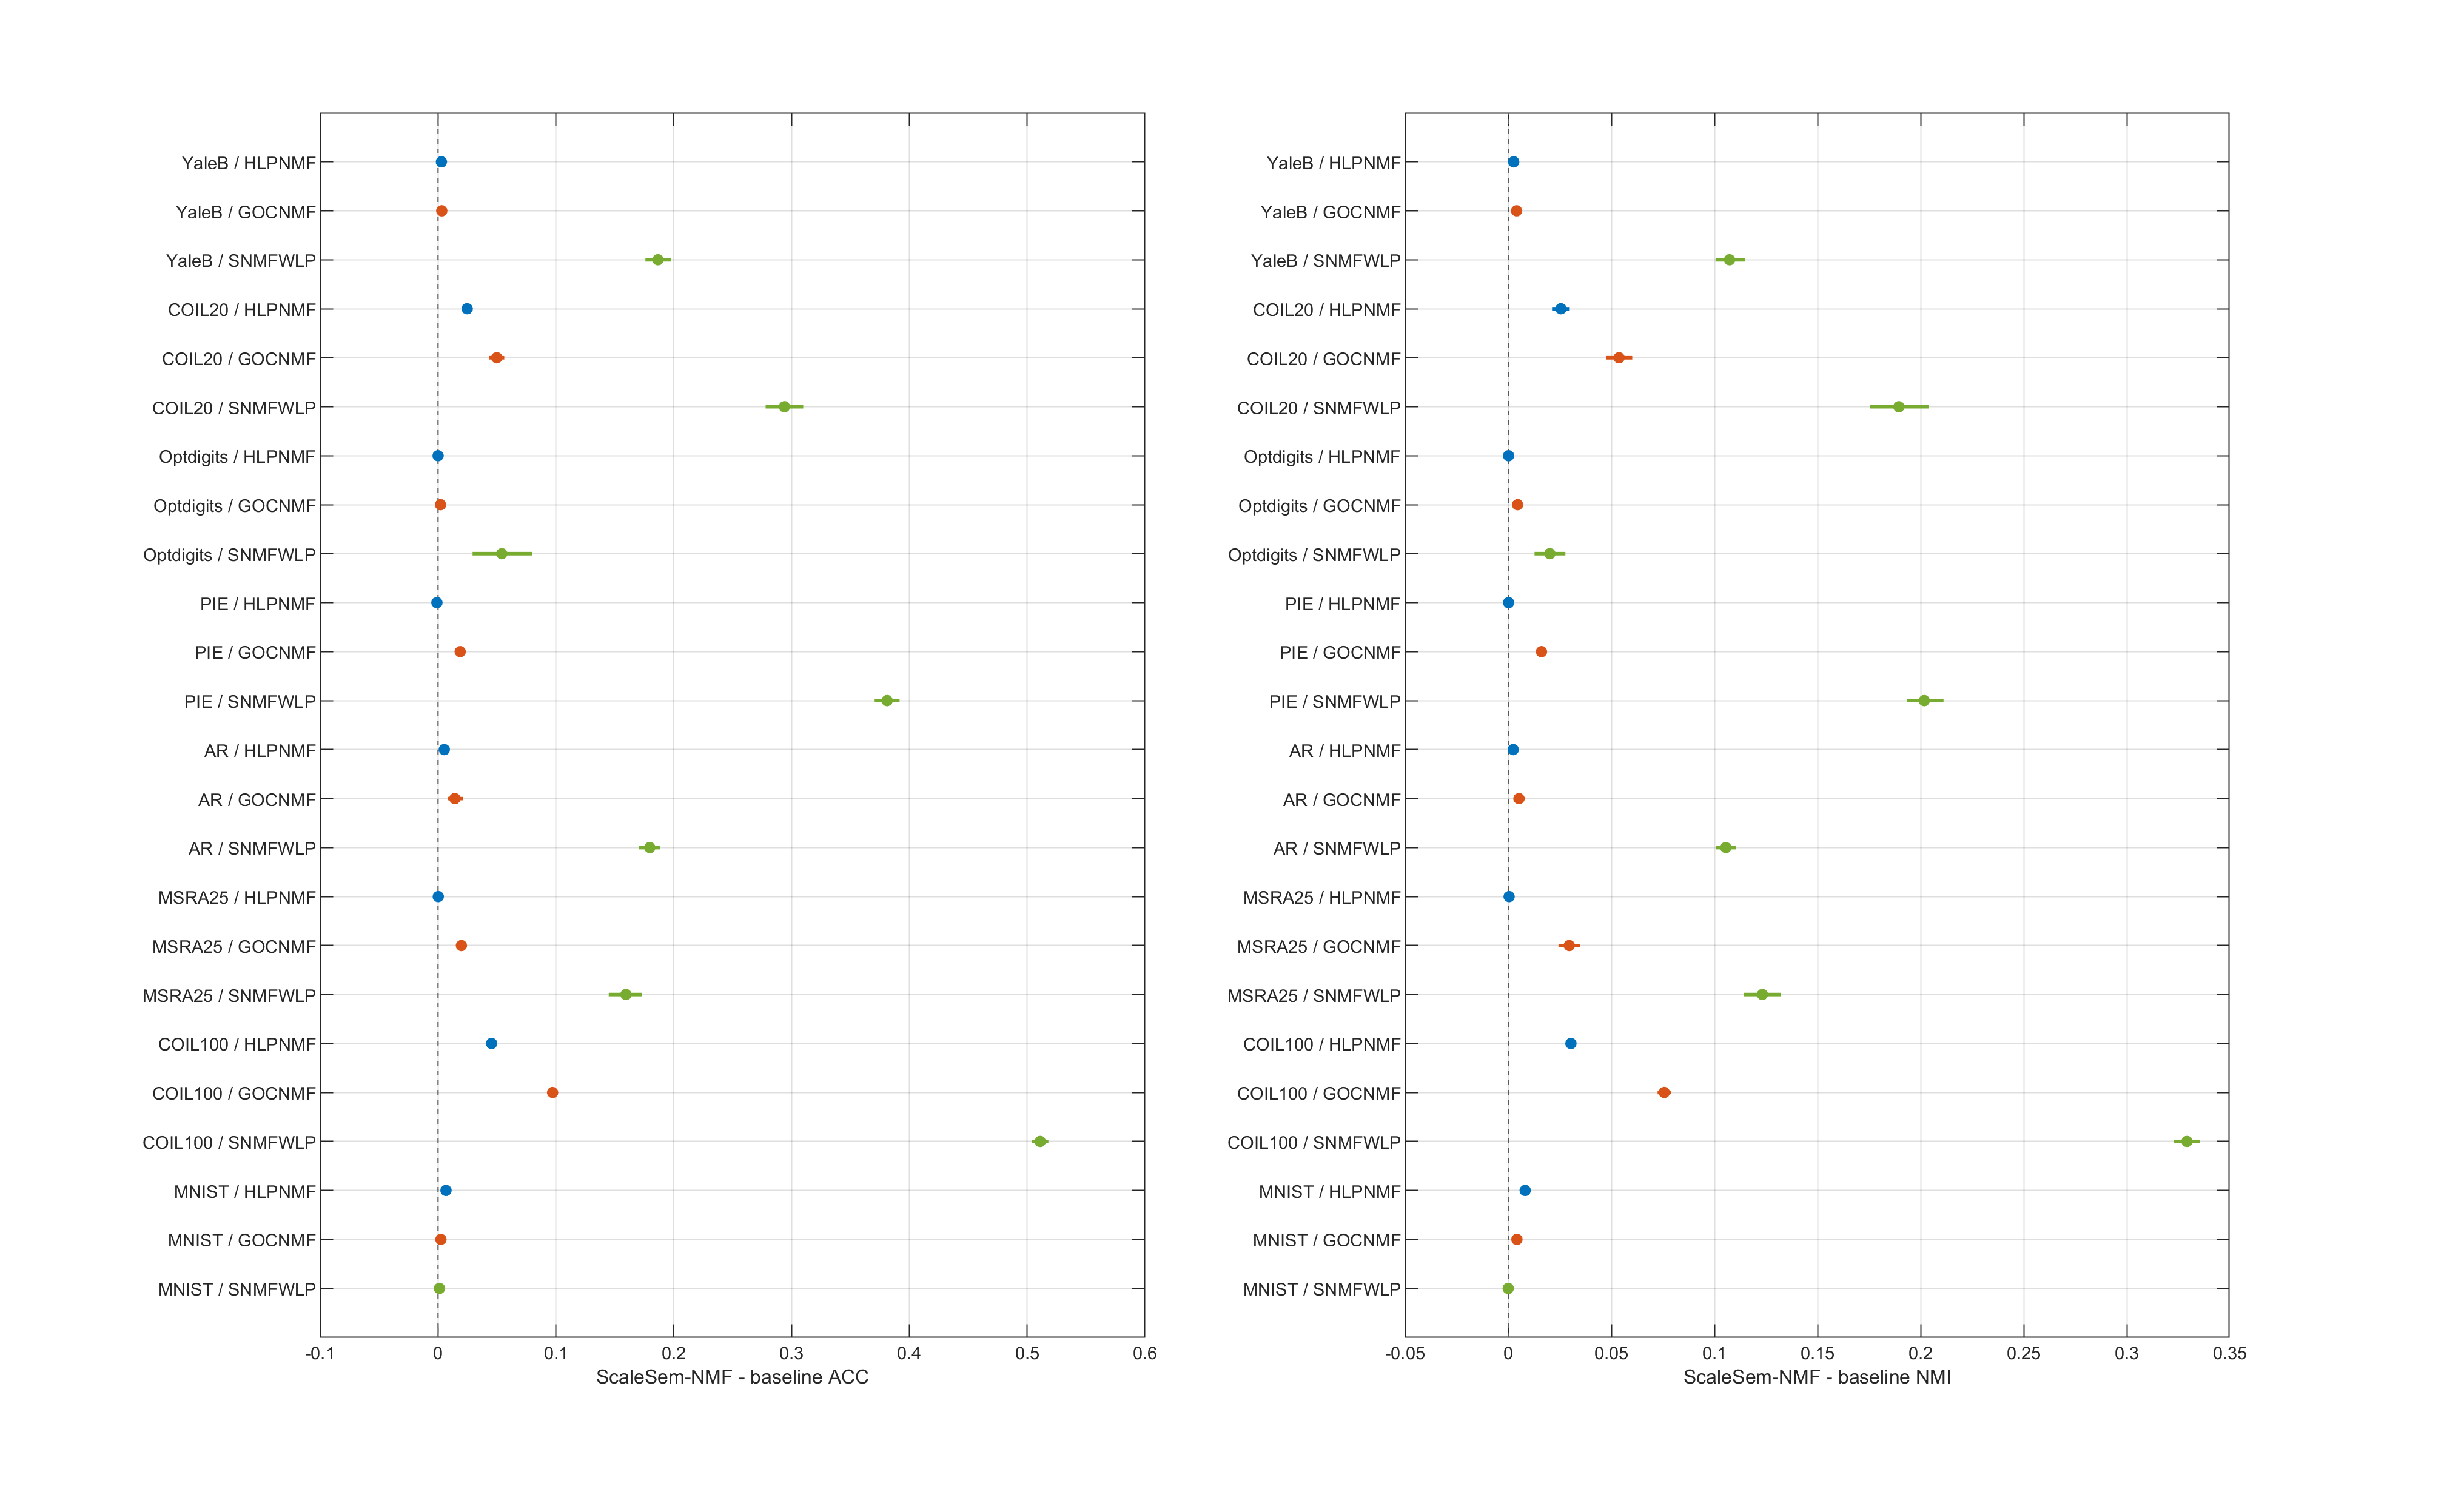
\includegraphics[width=0.96\textwidth,height=0.72\textheight,keepaspectratio]{figures/png/all8-paired-forest.png}
\caption{Paired ACC and NMI differences between ScaleSem-NMF and each baseline on all eight datasets. Points are mean paired differences and bars are 95\% percentile-bootstrap intervals from 10,000 resamples. Intervals crossing zero identify paired effects that include parity.}
\label{fig:paired}
\end{figure*}

Against all three baselines, the preregistered dual-metric paired-bootstrap criterion is satisfied on AR and COIL100. COIL100 also satisfies the 24-comparison Holm-adjusted sign tests throughout. AR is reported as a positive paired effect under the interval criterion.

\FloatBarrier
\subsection{Influence of supervision budget}

The supervision experiment contains 4 datasets $\times$ 5 ratios $\times$ 20 seeds $\times$ 4 methods = 1600 runs, with the ACC and NMI trajectories shown in Fig.~\ref{fig:labelratio}. Its preregistered low-label gate passes. At 5\% supervision, ScaleSem-NMF is within the dual-metric practical margin of the strongest baseline on PIE, MSRA25, and MNIST and is clearly stronger on COIL20. The same pattern holds at 15\%, demonstrating robustness across the tested supervision budgets.

\begin{figure*}[!htbp]
\centering
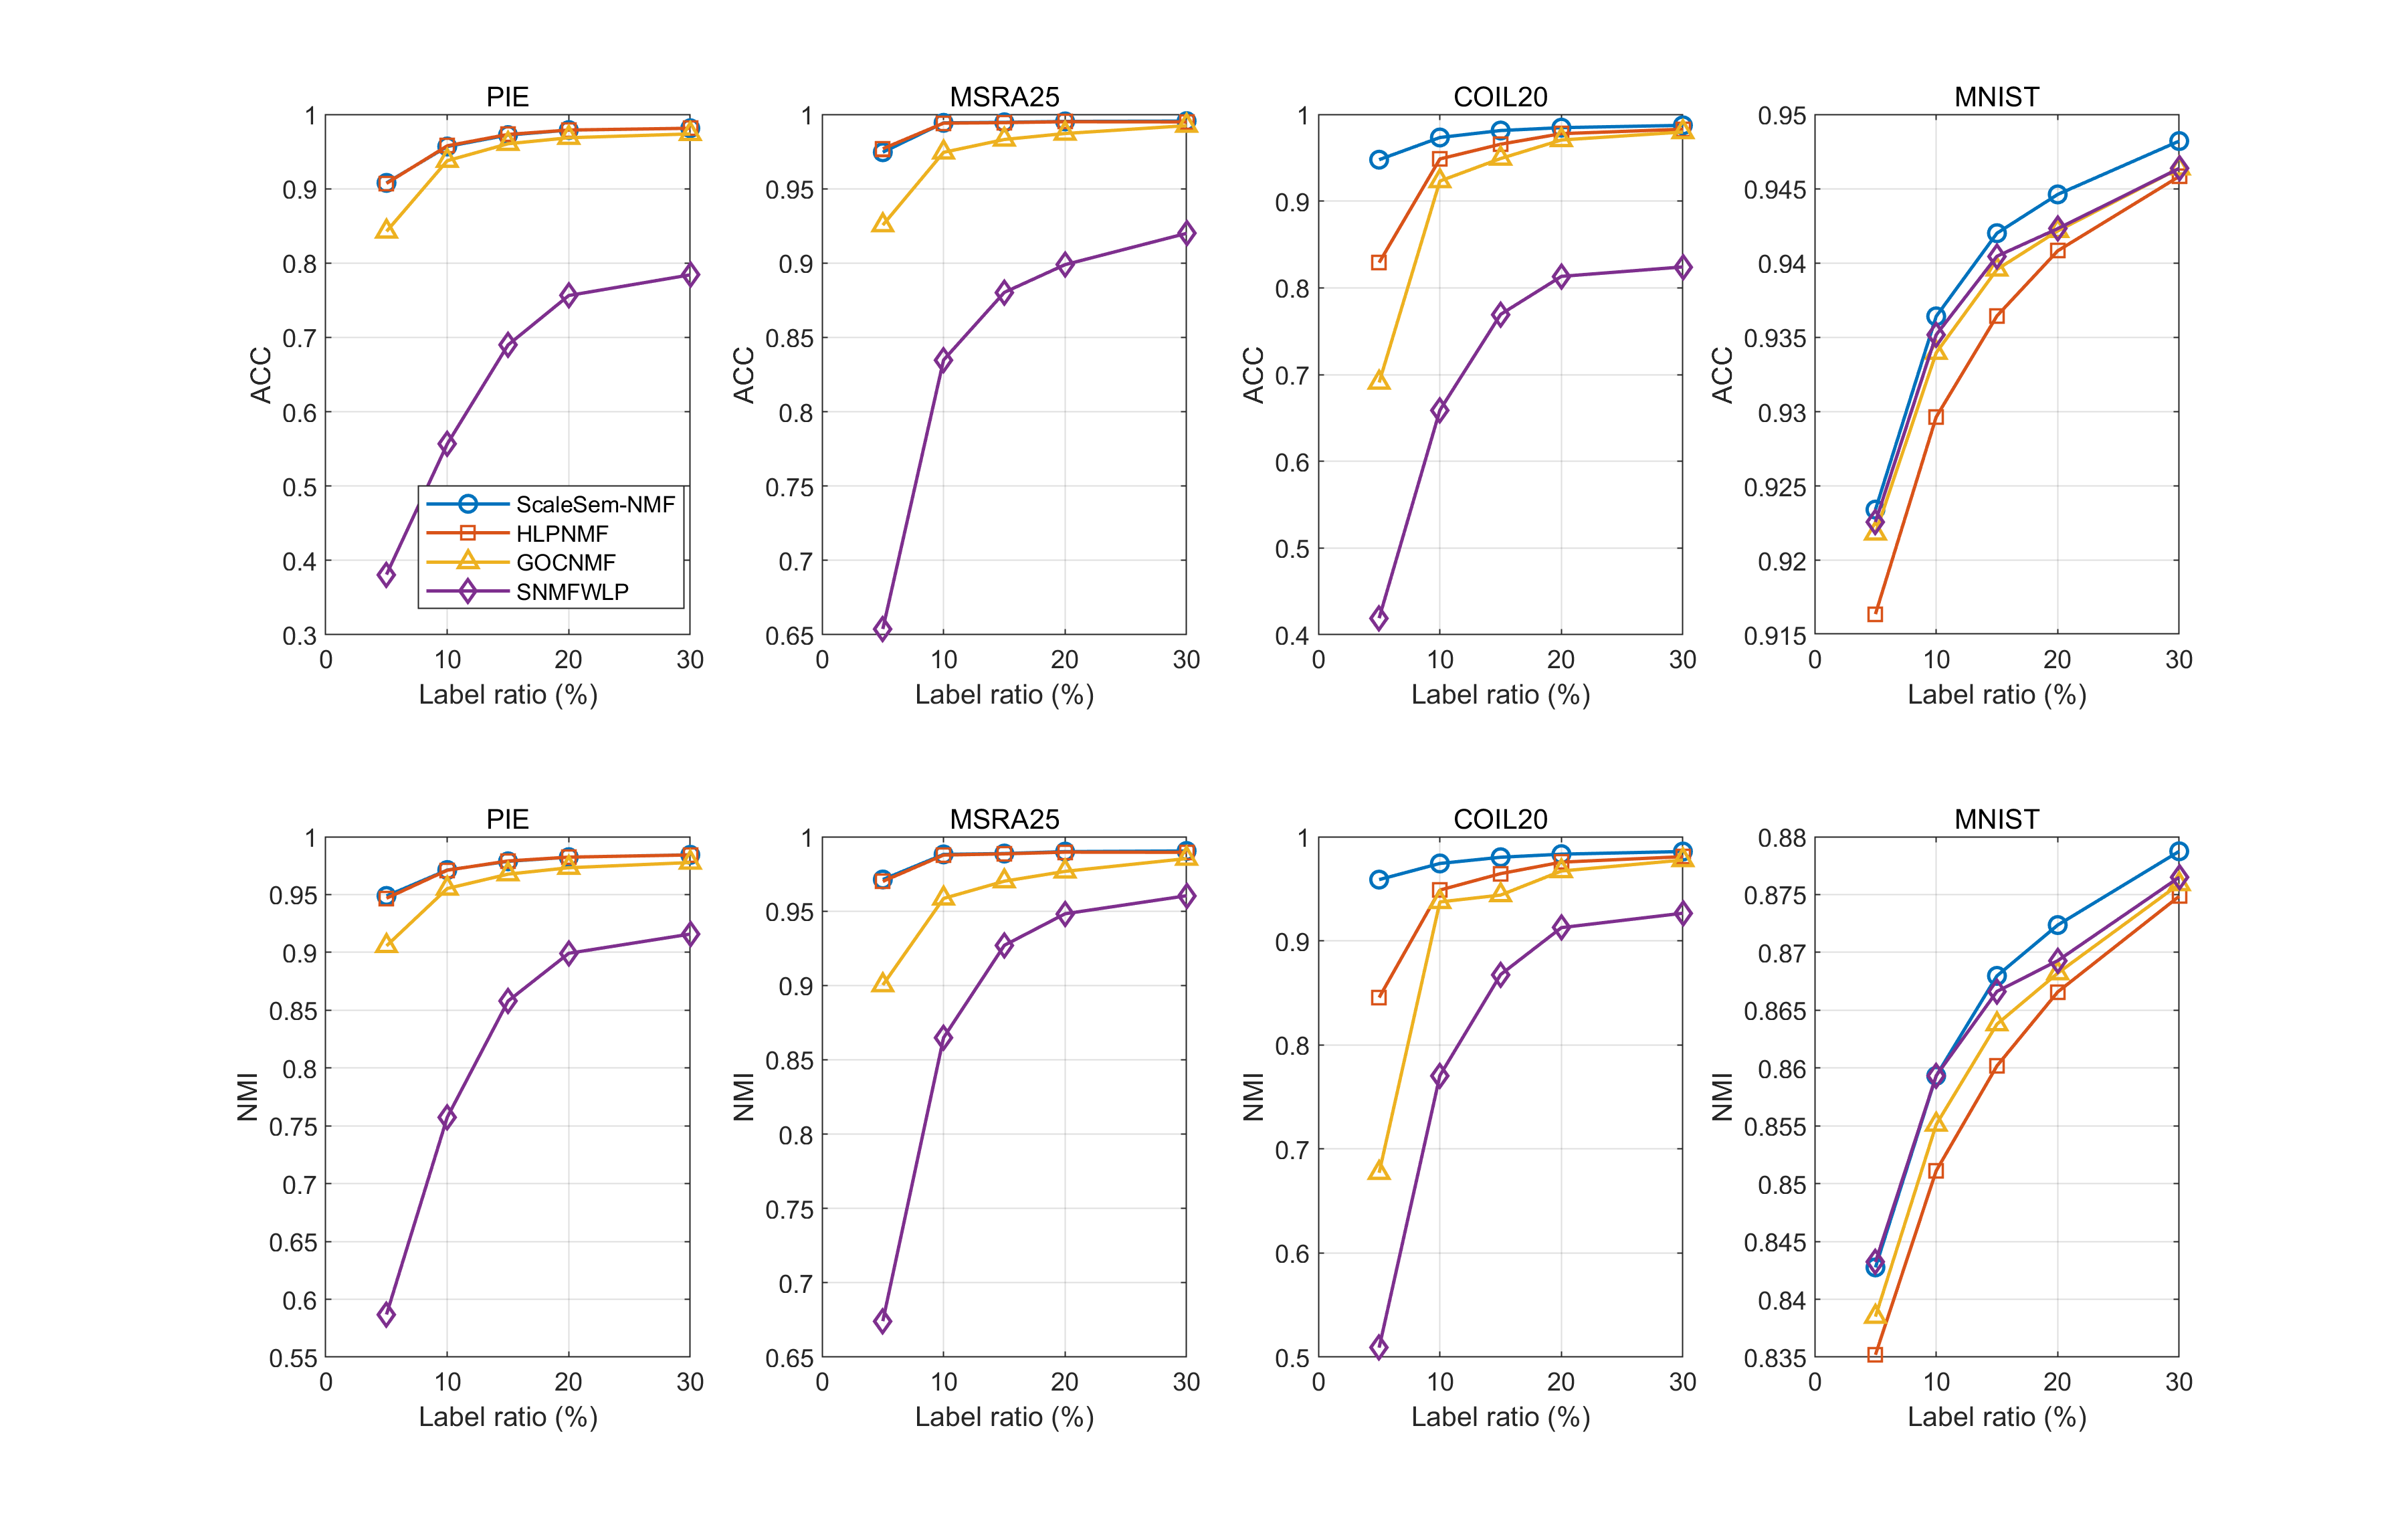
\includegraphics[width=0.90\textwidth,height=0.66\textheight,keepaspectratio]{figures/png/label-ratio.png}
\caption{ACC and NMI under the frozen supervision-budget protocol. Main-table parameters remain unchanged.}
\label{fig:labelratio}
\end{figure*}

\FloatBarrier
\subsection{Parameter sensitivity}

The sensitivity matrix contains 255 runs over COIL100, COIL20, and PIE; Fig.~\ref{fig:param} reports the corresponding ACC and NMI responses. The main-table parameters were unchanged. The regularization weight \(\alpha\) and propagation order \(k\) pass the preregistered local-stability threshold on all three datasets. Neighborhood size \(p\) shows the strongest sensitivity, with worst median ACC losses of 0.511, 0.448, and 0.148, respectively, making graph-neighborhood selection an important practical consideration.

\begin{figure*}[!htbp]
\centering
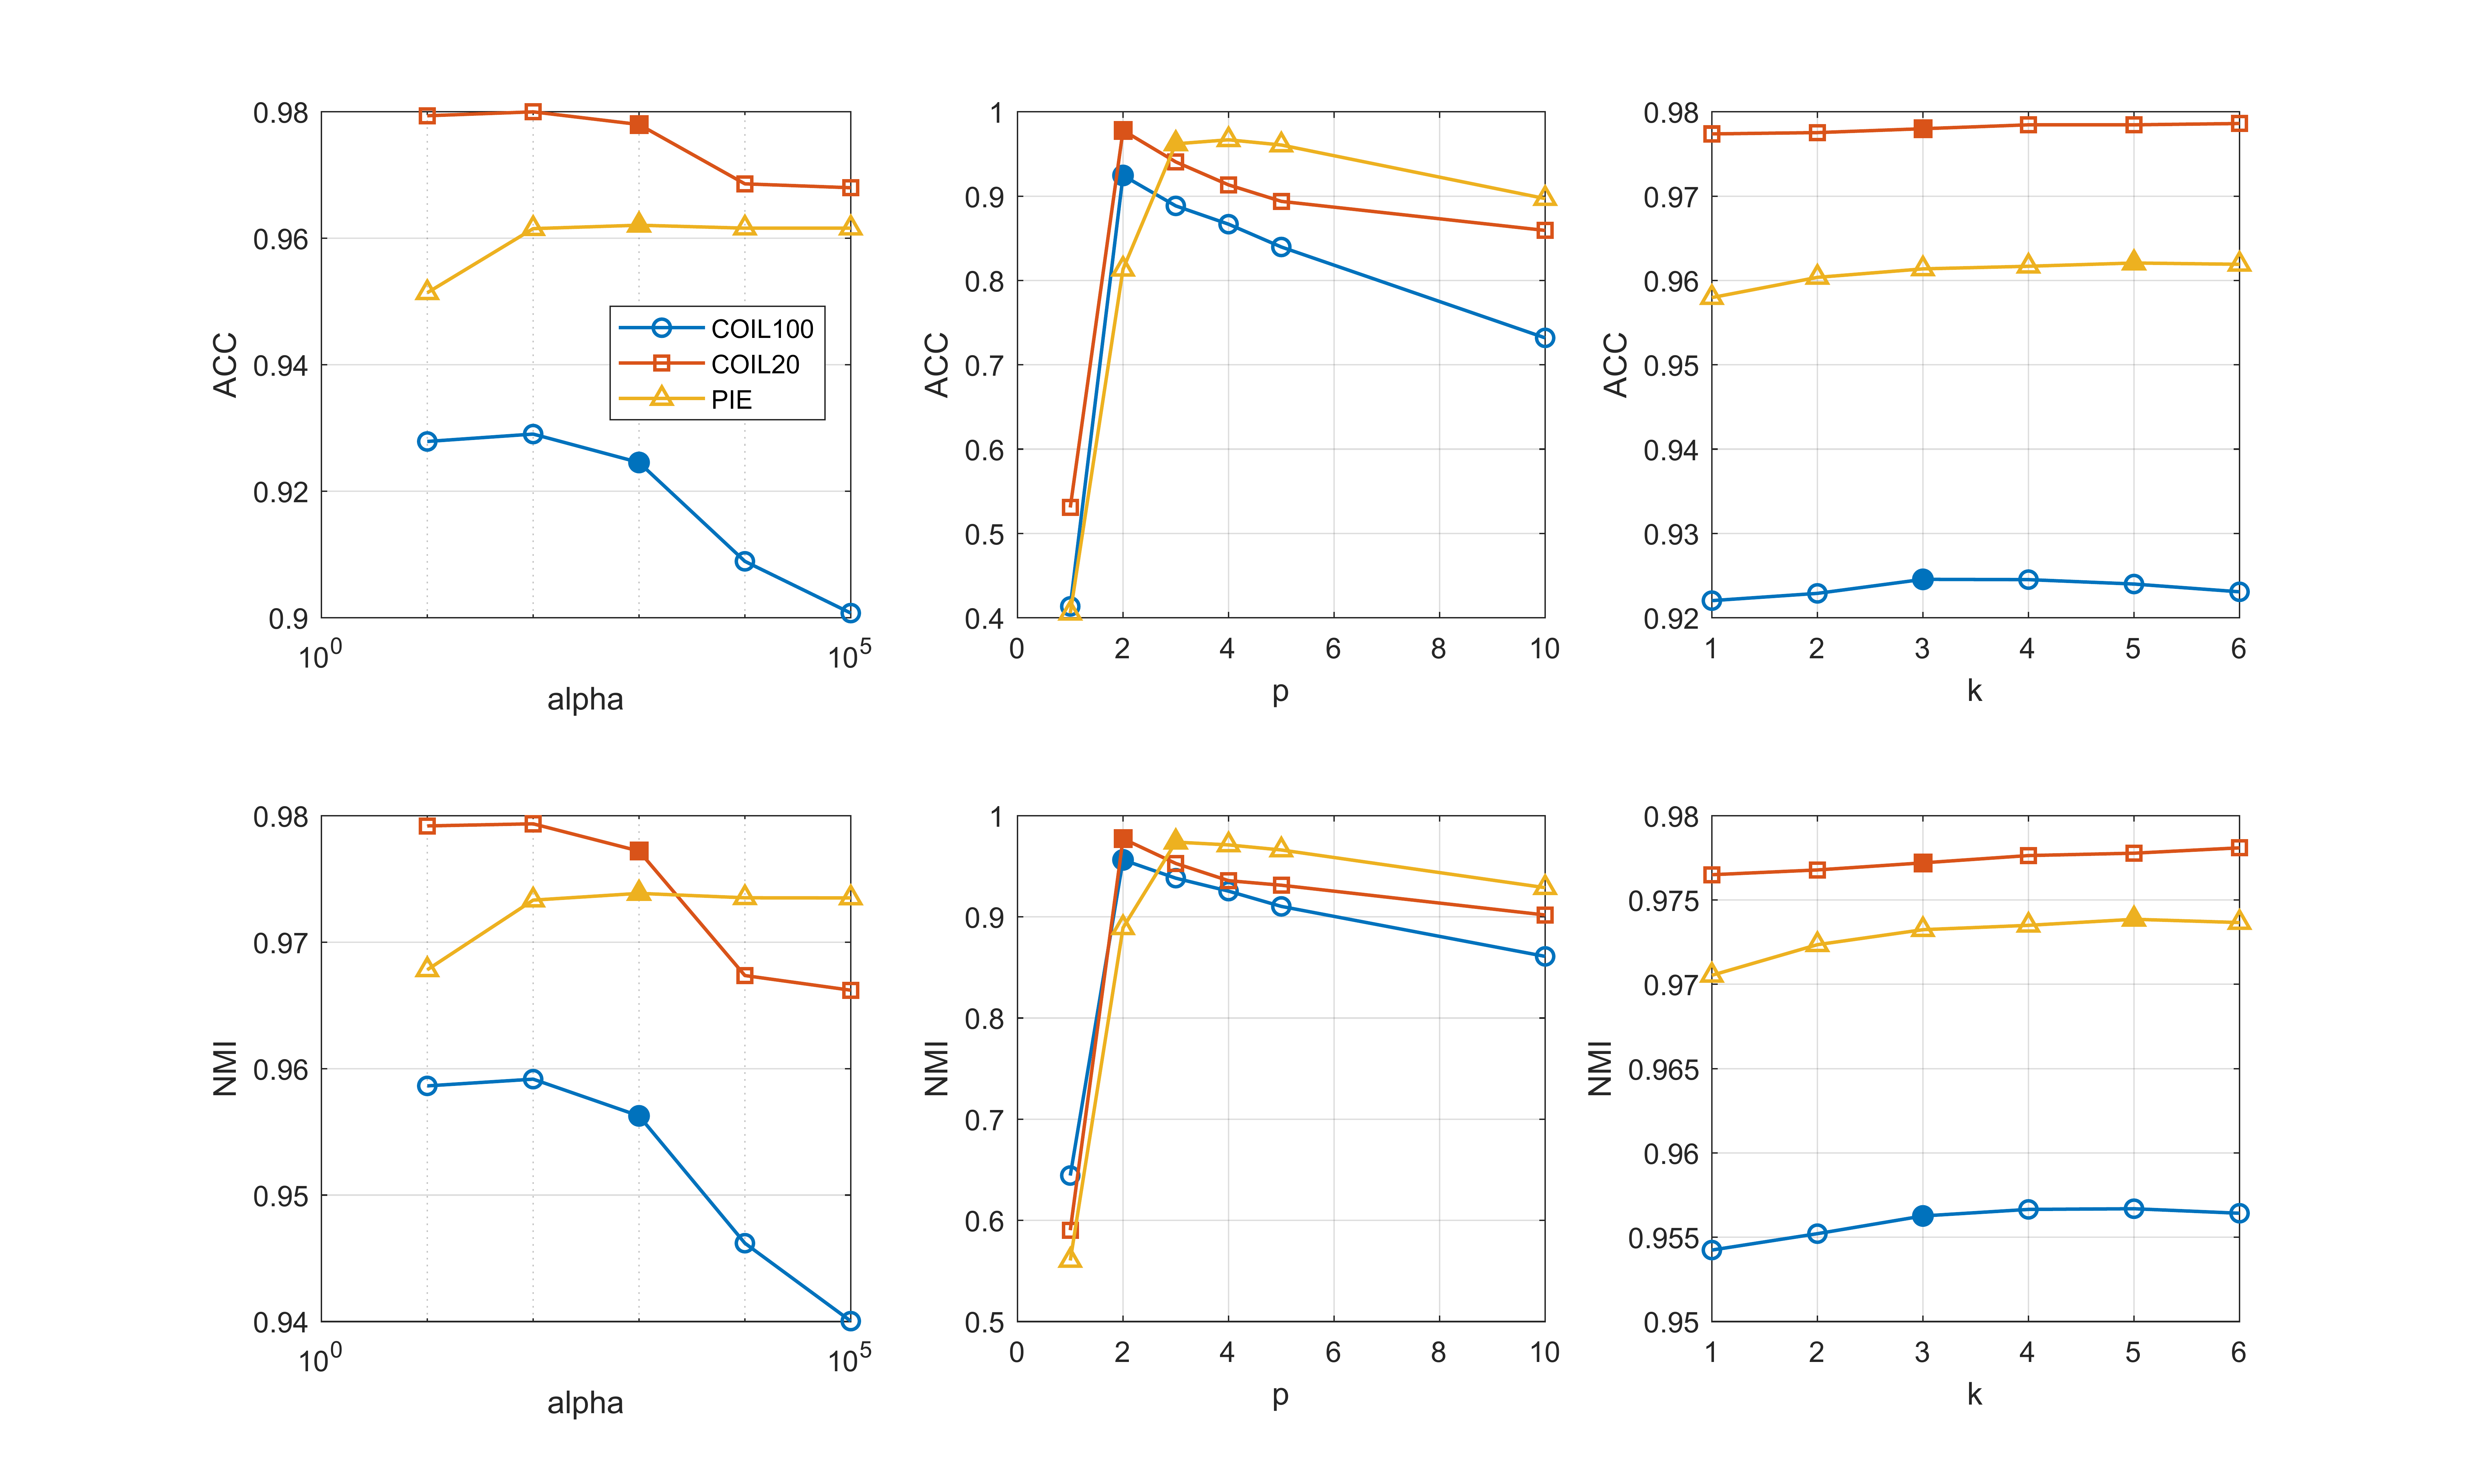
\includegraphics[width=0.87\textwidth,height=0.62\textheight,keepaspectratio]{figures/png/parameter-sensitivity.png}
\caption{Parameter sensitivity of ScaleSem-NMF for ACC and NMI.}
\label{fig:param}
\end{figure*}

\FloatBarrier
\subsection{Salt-and-pepper robustness}

The formal noise matrix contains 400 unique runs. For salt-and-pepper corruption, the same corrupted images and pixels were shared across methods within each paired cell. Figure~\ref{fig:noise} reports the performance curves. The main gate required ScaleSem-NMF to remain within 0.01 ACC and NMI of the strongest baseline on at least two datasets at every level from 10\% through 30\%. COIL20, PIE, and YaleB all pass individually, so the overall gate passes.

\begin{figure*}[!htbp]
\centering
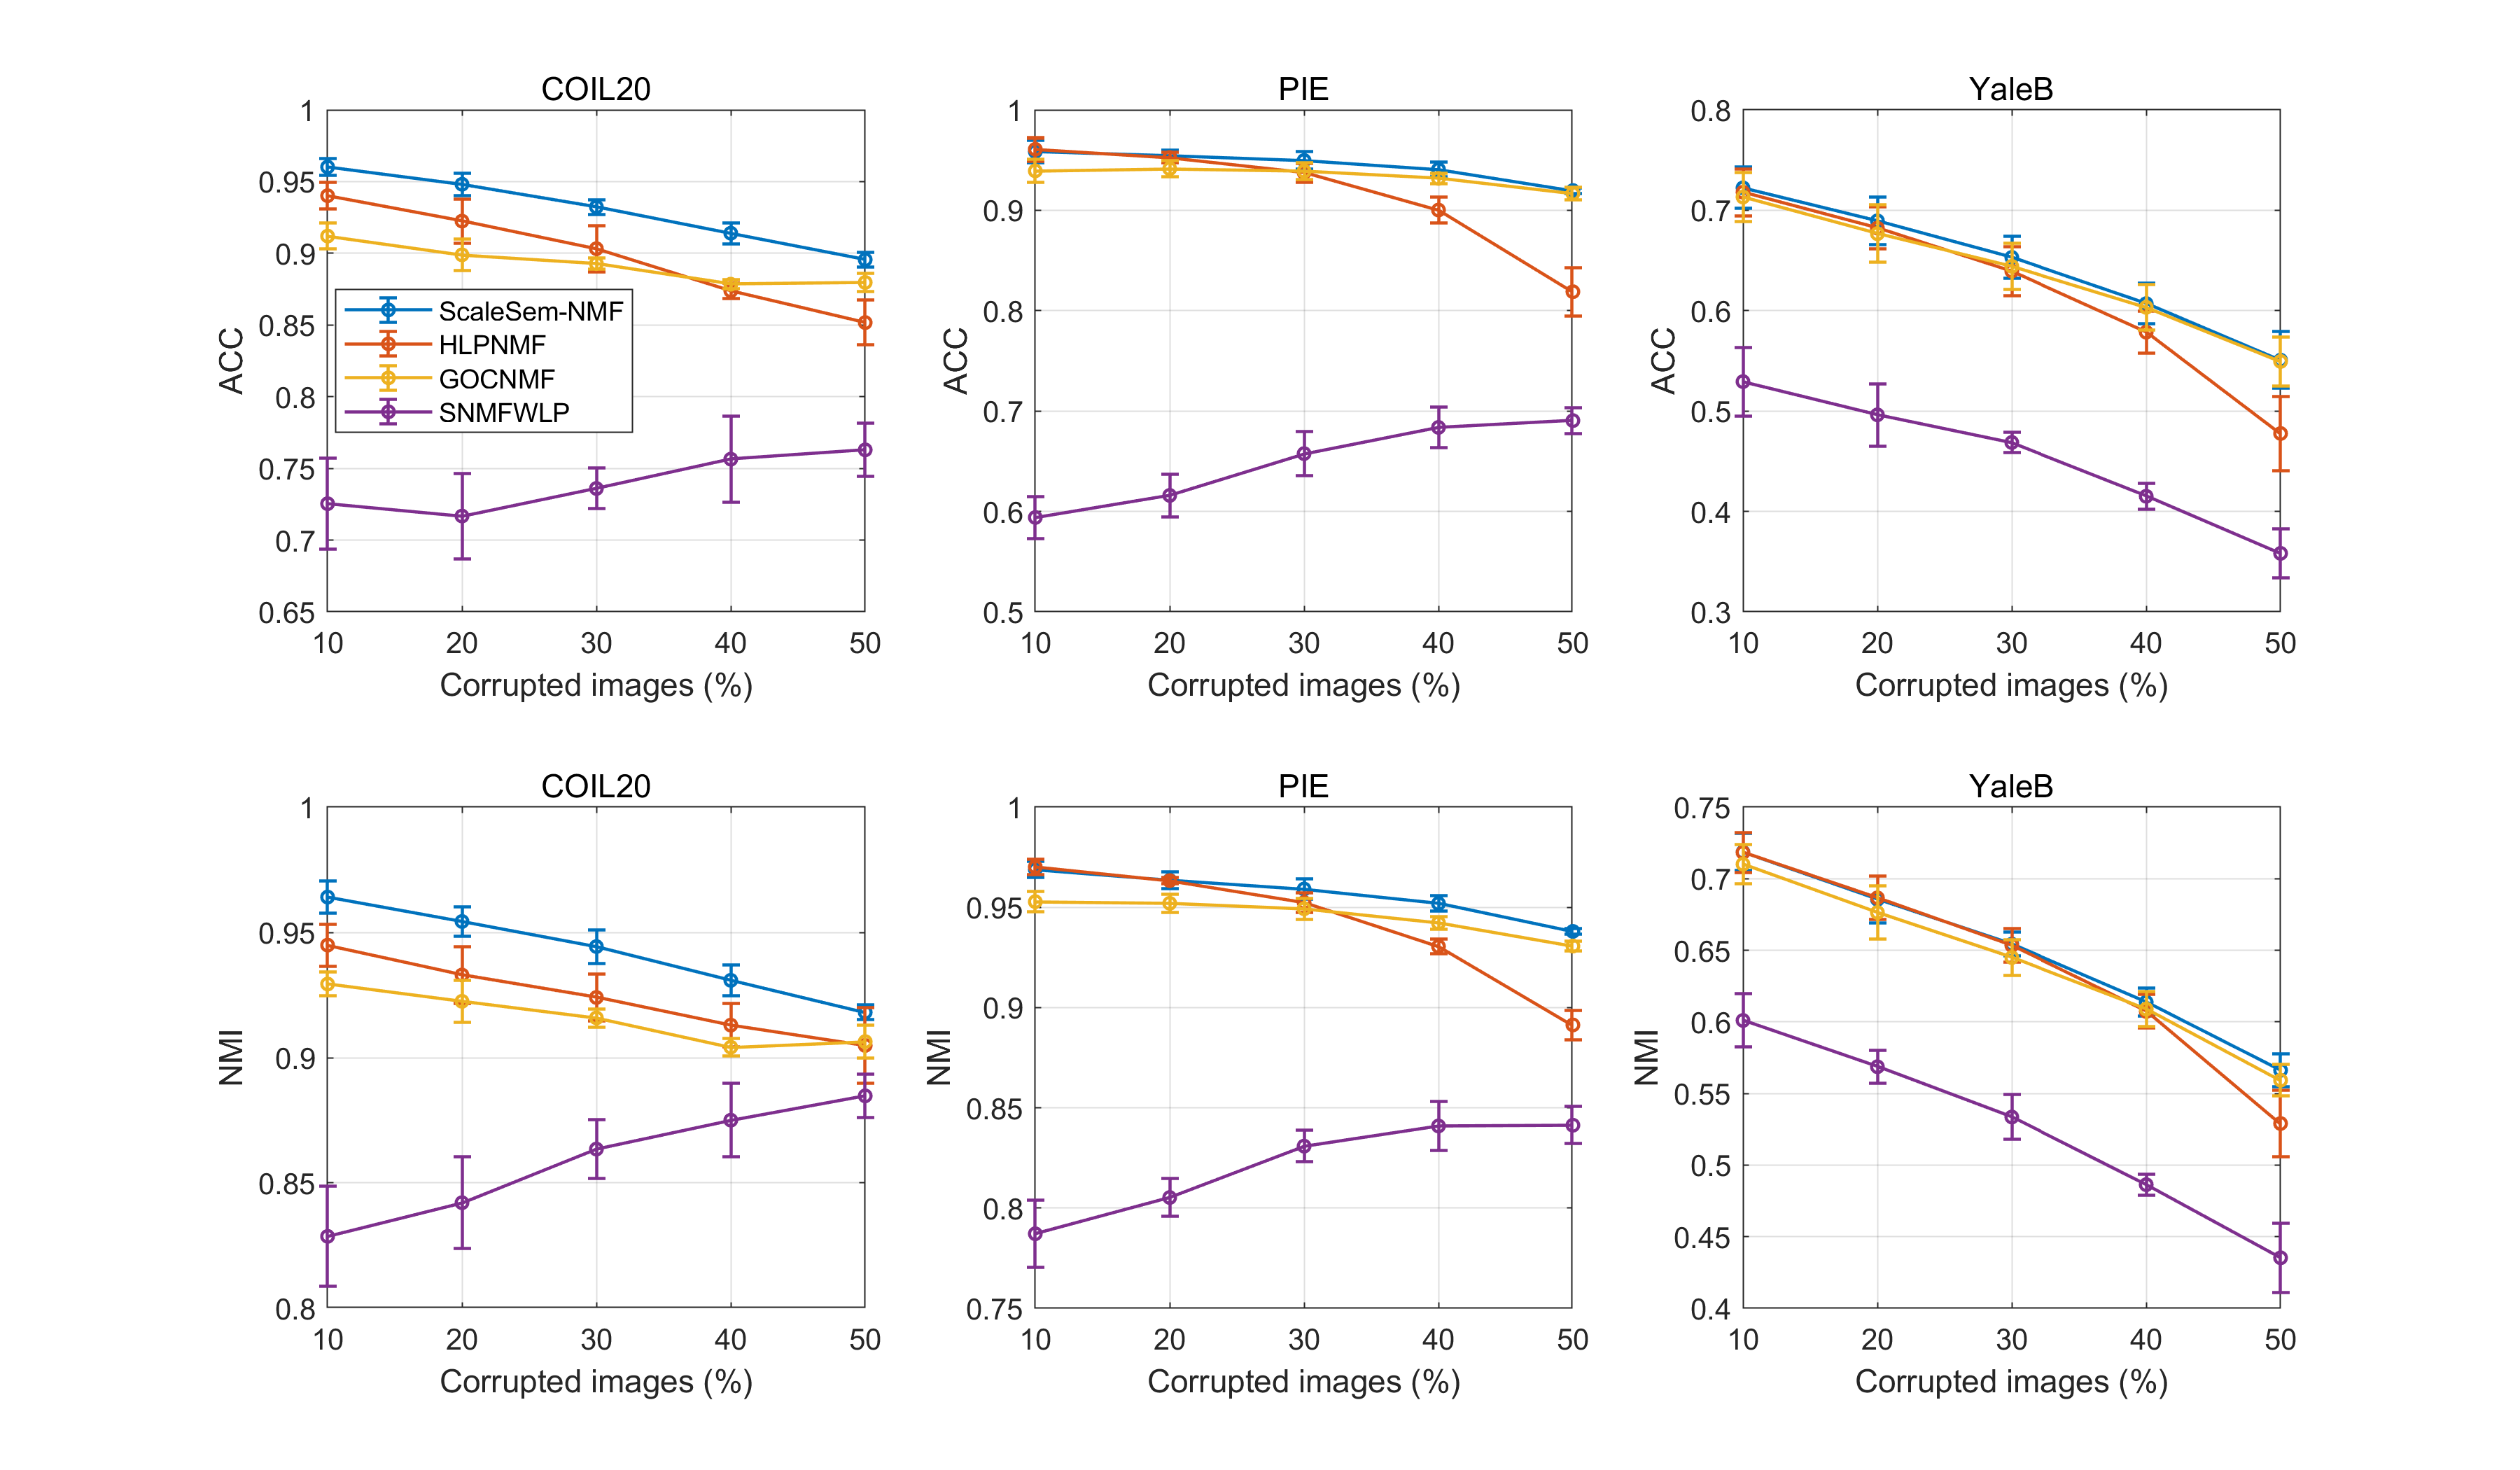
\includegraphics[width=0.90\textwidth,height=0.66\textheight,keepaspectratio]{figures/png/noise-robustness.png}
\caption{Salt-and-pepper robustness on three datasets.}
\label{fig:noise}
\end{figure*}

\FloatBarrier

At 30\% corruption, ScaleSem-NMF exceeds the strongest baseline by 0.0291 ACC and 0.0203 NMI on COIL20; by 0.0107 ACC and 0.0067 NMI on PIE; and by 0.0089 ACC and 0.0009 NMI on YaleB. The 40\% and 50\% points are stress tests and do not redefine the gate.

Figure~\ref{fig:corruption_examples} shows reproducible examples from the formal protocol rather than separately designed illustrations. For seed 20260627, 30\% of samples are selected by the same deterministic random process used in evaluation, and exactly 10\% of the 32-by-32 pixels in every selected image are replaced by balanced zero/255 impulses.

\begin{figure}[H]
\centering
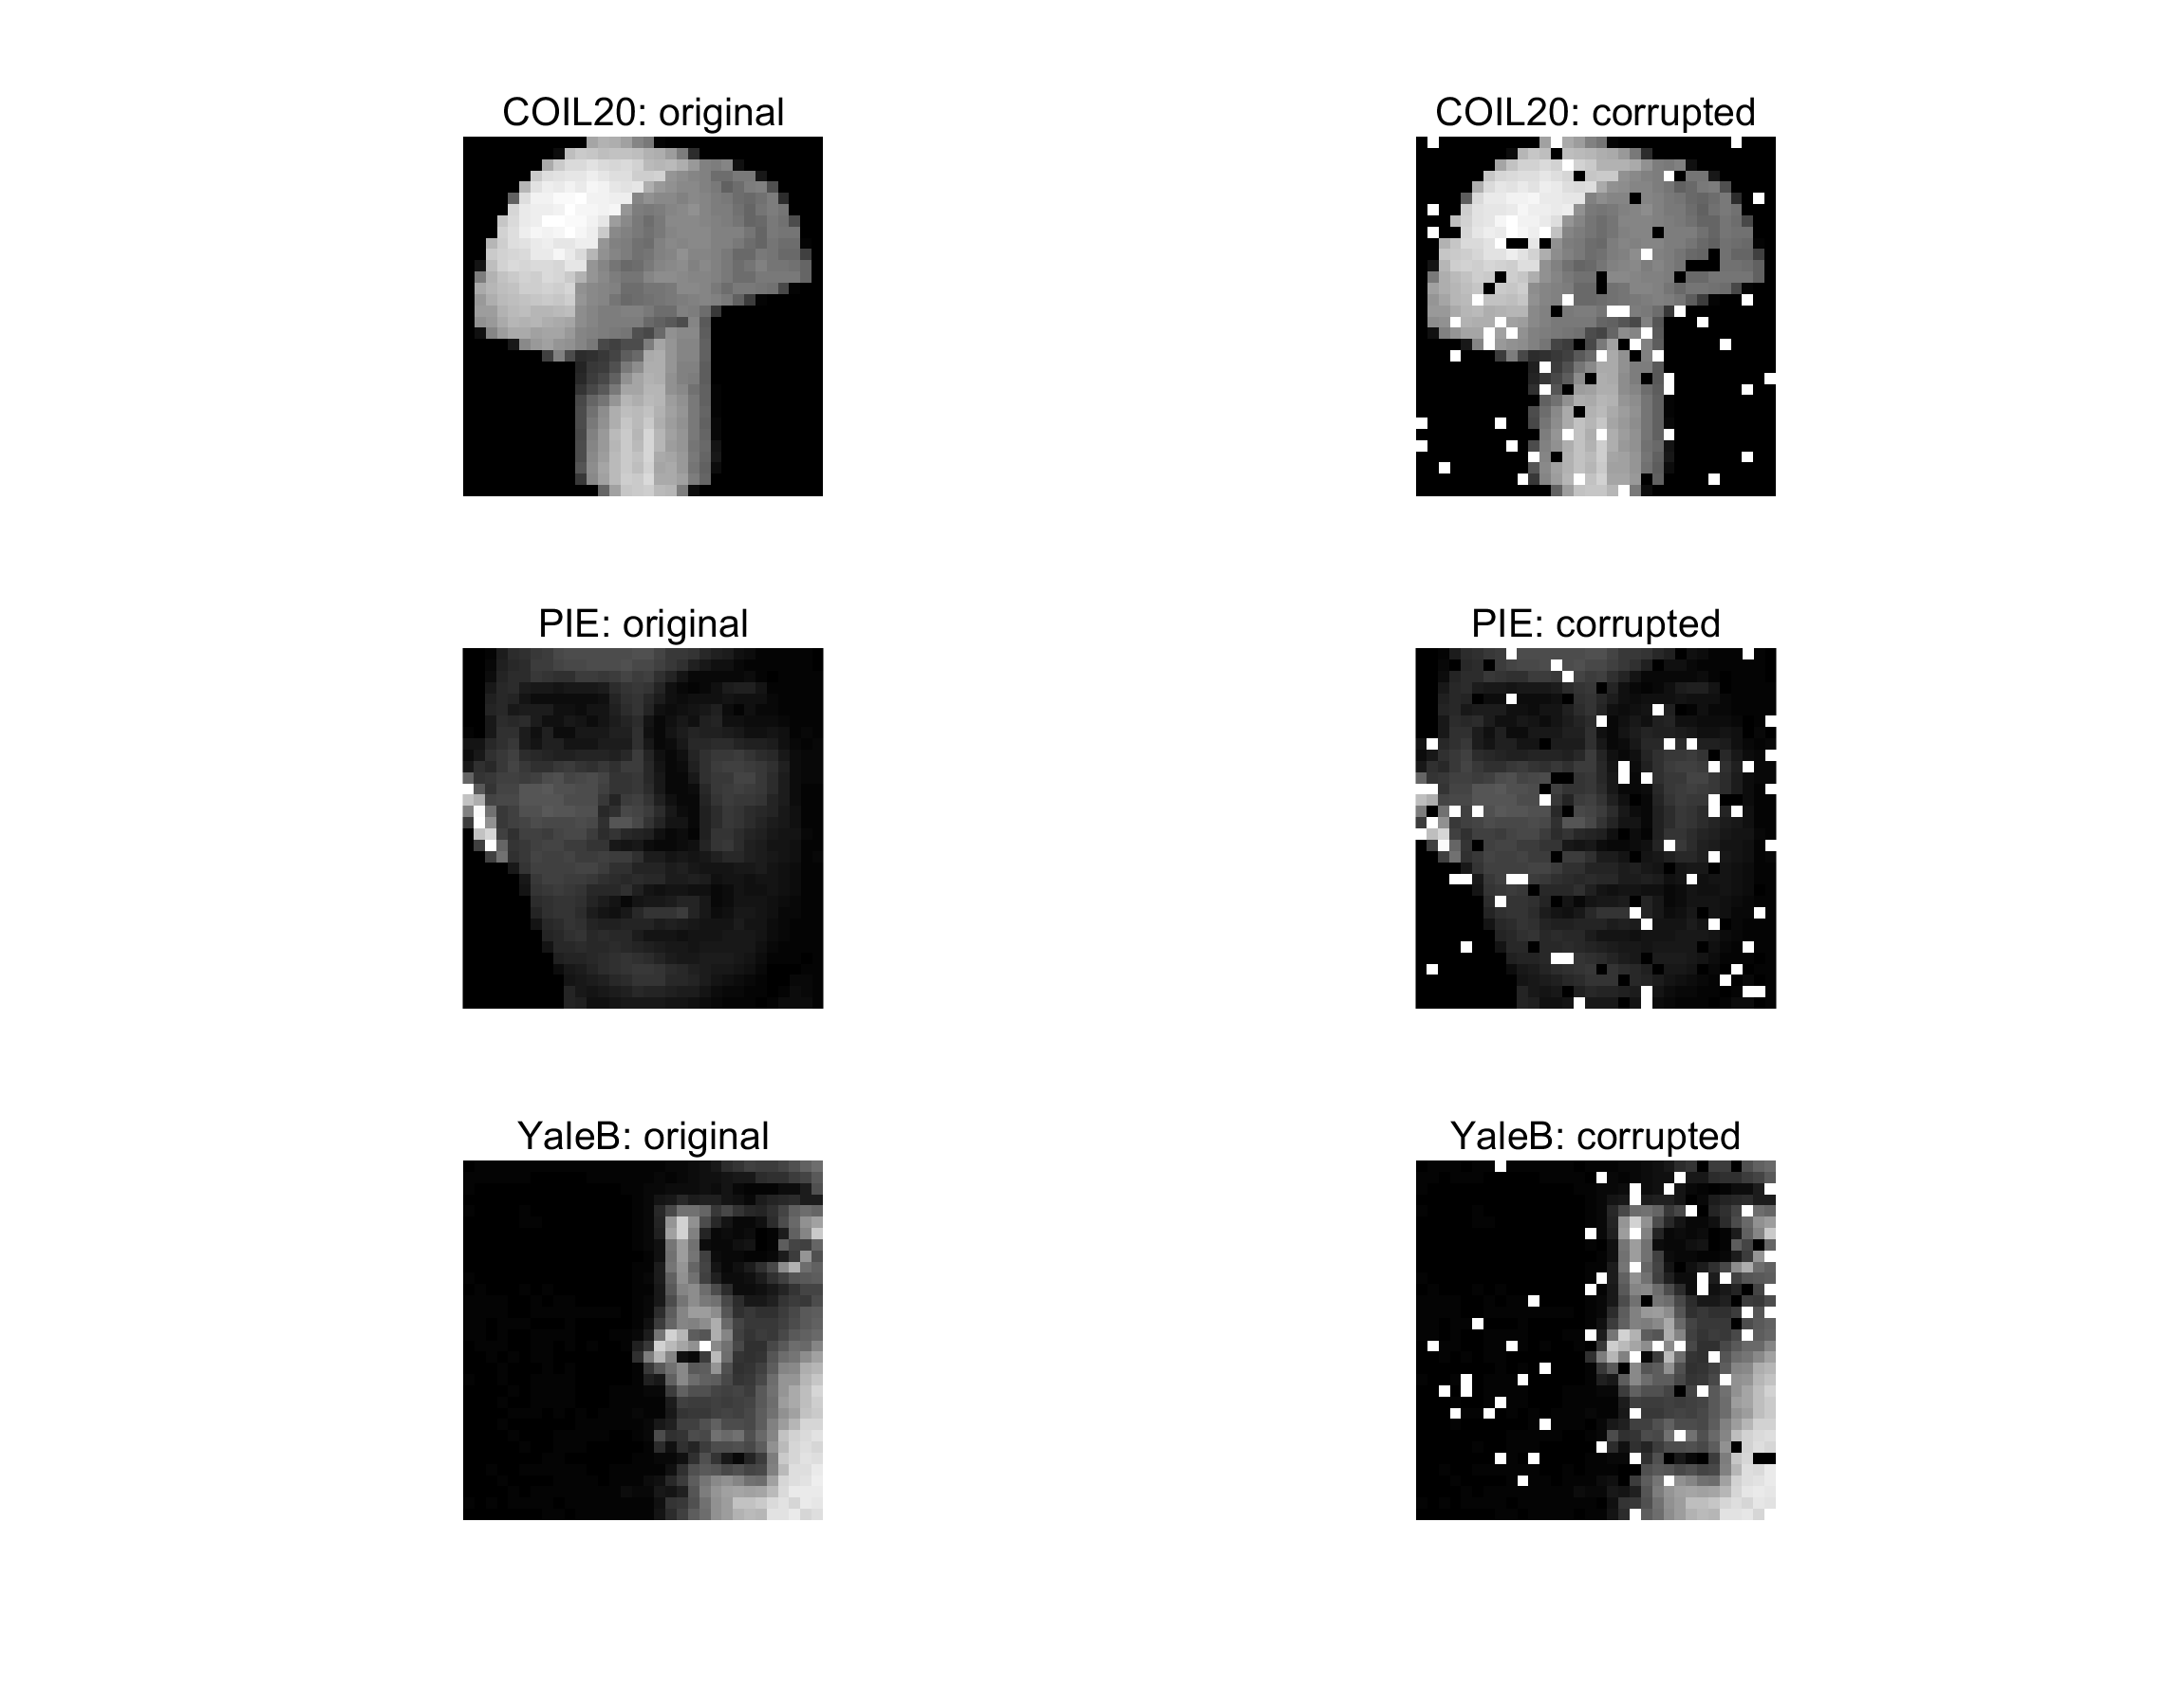
\includegraphics[width=0.88\columnwidth,height=0.58\textheight,keepaspectratio]{figures/png/corruption-examples.png}
\caption{Examples of the salt-and-pepper corruption used in the formal robustness experiment. Each row shows the same selected sample before and after corruption.}
\label{fig:corruption_examples}
\end{figure}

\FloatBarrier
\subsection{Unified single-thread runtime}

The unified runtime matrix contains 8 datasets $\times$ 4 methods $\times$ 5 paired seeds = 160 runs in one MATLAB R2019a process with `-singleCompThread`. Figure~\ref{fig:runtime} shows the runtime distributions, and Table~\ref{tab:runtime} gives the paired medians. Timing includes graph construction, native optimization, and native decision, while excluding data loading, normalization, split generation, metric calculation, and file writing. The preregistered speed gate required a lower paired median on at least 6 of 8 datasets.

\begin{figure*}[!htbp]
\centering
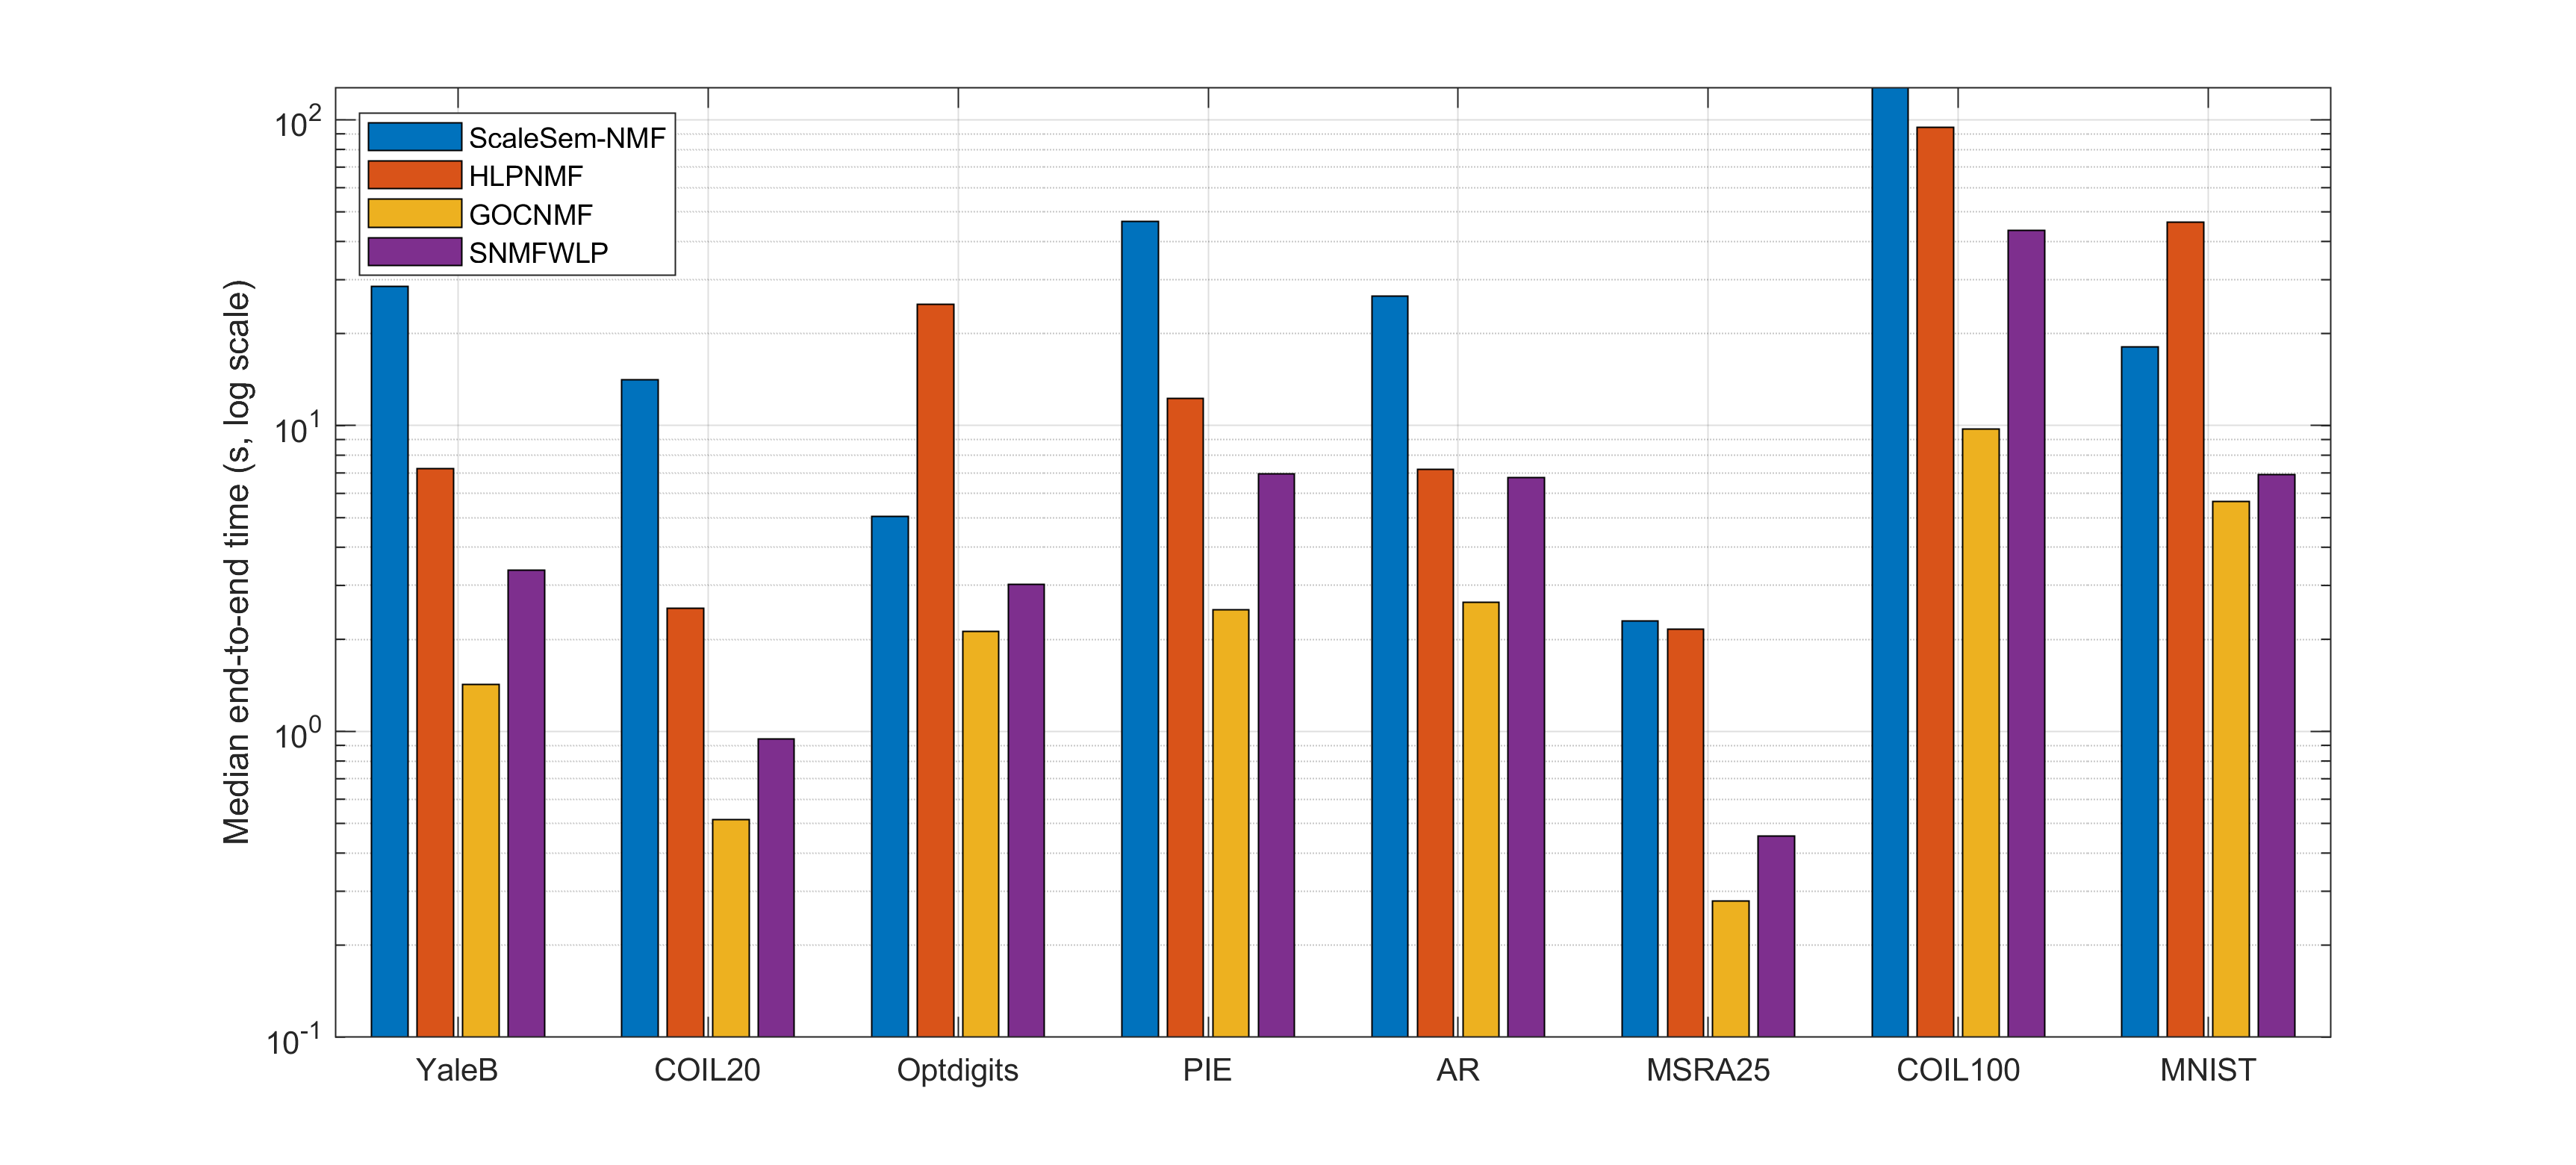
\includegraphics[width=0.90\textwidth,height=0.64\textheight,keepaspectratio]{figures/png/unified-runtime.png}
\caption{Unified single-thread runtime comparison.}
\label{fig:runtime}
\end{figure*}

\begin{table*}[!htbp]
\centering
\caption{Median unified single-thread runtime in seconds over five paired seeds. Lower is better.}
\label{tab:runtime}
\scriptsize
\begin{tabular}{lrrrr}
\toprule
Dataset & ScaleSem-NMF & HLPNMF & GOCNMF & SNMFWLP \\
\midrule
YaleB & 28.510 & 7.221 & \textbf{1.426} & 3.364 \\
COIL20 & 14.152 & 2.523 & \textbf{0.513} & 0.943 \\
Optdigits & 5.058 & 24.905 & \textbf{2.122} & 3.027 \\
PIE & 46.429 & 12.257 & \textbf{2.493} & 6.967 \\
AR & 26.544 & 7.185 & \textbf{2.646} & 6.742 \\
MSRA25 & 2.295 & 2.163 & \textbf{0.279} & 0.454 \\
COIL100 & 127.559 & 94.454 & \textbf{9.771} & 43.380 \\
MNIST & 18.082 & 46.196 & \textbf{5.662} & 6.896 \\
\bottomrule
\end{tabular}
\end{table*}

ScaleSem-NMF is faster than HLPNMF on 2 of 8 datasets. GOCNMF and SNMFWLP have lower runtimes across the tested datasets. These measurements quantify the computational profile associated with the observed clustering and salt-and-pepper results.

\FloatBarrier
\subsection{PIE scale and retained graph storage}

Nested PIE subsets contain 10, 20, 40, and 68 classes with 420, 840, 1680, and 2856 samples. Figure~\ref{fig:scale} summarizes performance, runtime, and retained graph storage as the subset grows. All 20 runs are finite and monotone. Median runtime grows from 3.58 s to 43.96 s, while measured retained graph storage grows to 6.07 MiB on full PIE. Descriptive log-log slopes are 1.298 for runtime and 1.133 for retained graph storage over these four points. These measurements characterize computational feasibility through full PIE.

\begin{figure*}[!htbp]
\centering
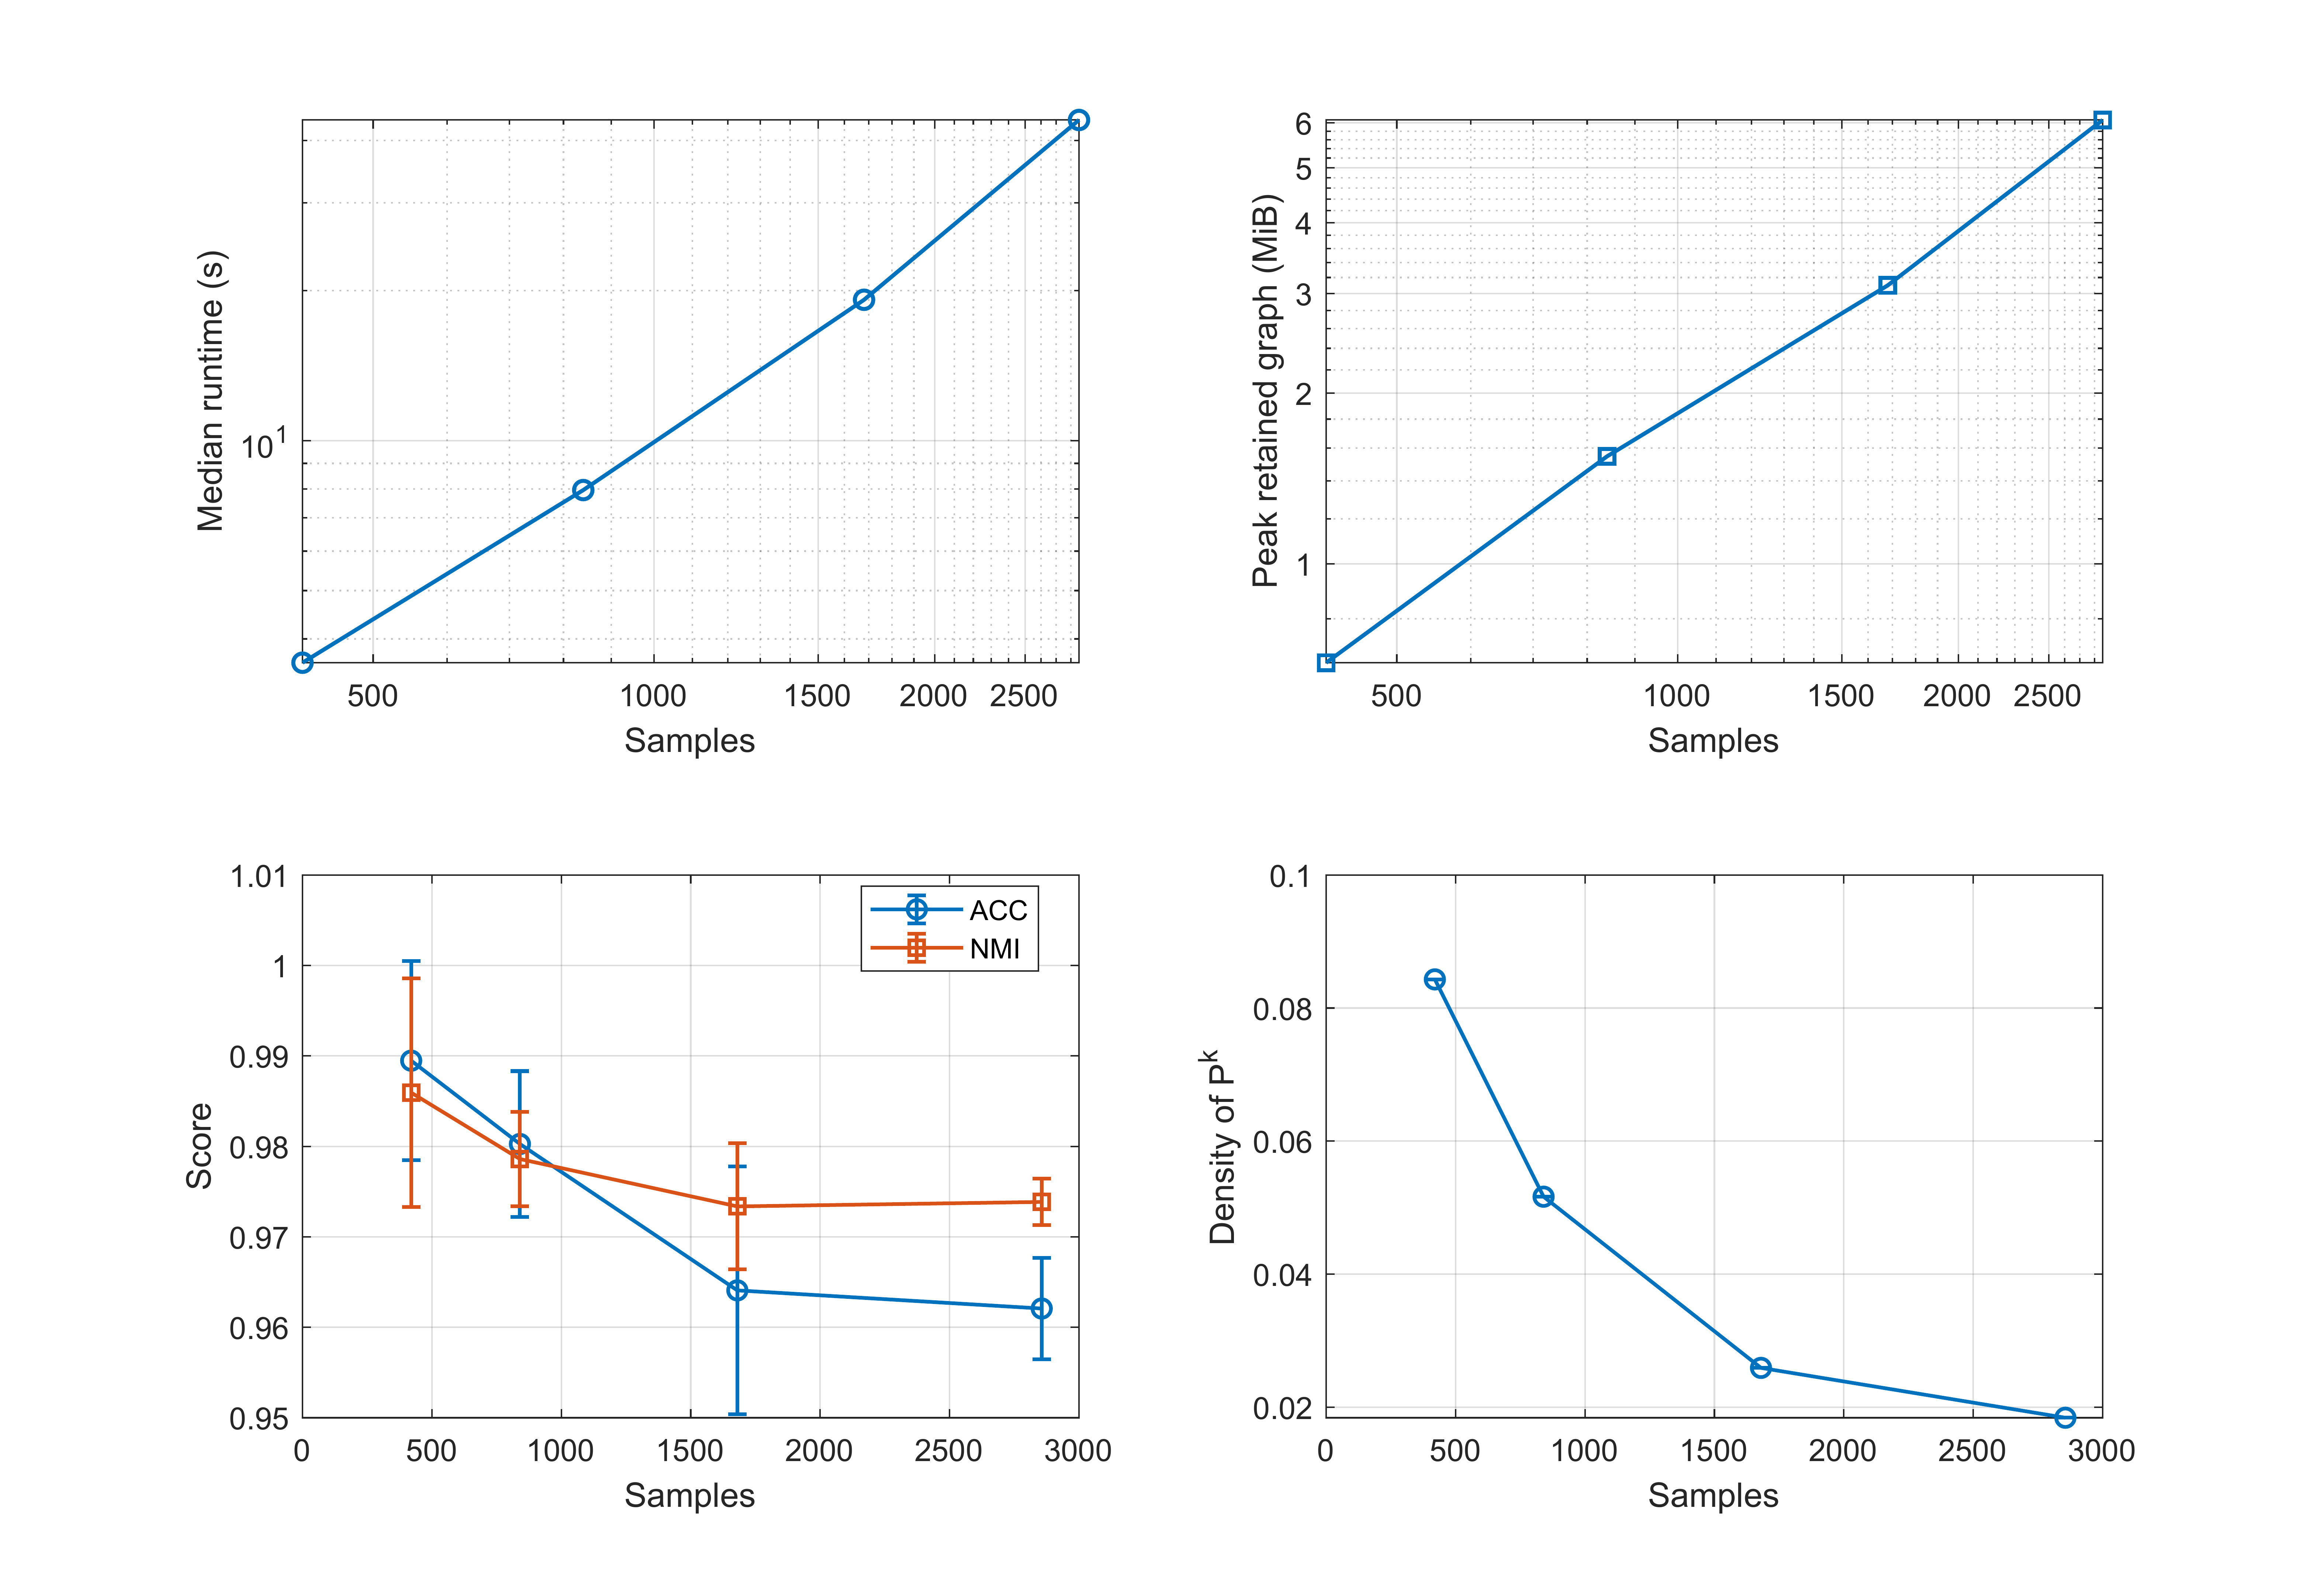
\includegraphics[width=0.90\textwidth,height=0.66\textheight,keepaspectratio]{figures/png/pie-scalability.png}
\caption{PIE scale, runtime, and retained graph storage through the full dataset.}
\label{fig:scale}
\end{figure*}

\FloatBarrier
\subsection{Controlled mechanism ablations}

Table~\ref{tab:ablation_design} defines the two controlled variants. Each changes one role of the complete model while retaining the frozen split, graph, supervision budget, parameter setting, initialization contract, and stopping rule. Thus the full-minus-variant differences isolate adaptive amplitude and reconstruction coupling under the tested implementation; they are not comparisons against retuned alternative models.

\begin{table*}[!htbp]
\centering
\caption{Controlled ScaleSem-NMF ablation design. Only the stated mechanism is removed; all evaluation and graph settings remain frozen.}
\label{tab:ablation_design}
\small
\resizebox{\textwidth}{!}{%
\begin{tabular}{llll}
\toprule
Variant & Sample amplitude $s$ & Reconstruction contribution & Semantic propagation \\
\midrule
Full ScaleSem-NMF & learned by exact nonnegative update & retained & retained \\
Fixed-scale & fixed for all samples & retained & retained \\
Propagation-only & not optimized (irrelevant) & removed & retained \\
\bottomrule
\end{tabular}
}
\end{table*}

Adaptive scale and reconstruction coupling both provide stable incremental value on COIL100, and the earlier protocol shows a strong effect on COIL20. Their effects are smaller on the remaining datasets, indicating that the contribution of each mechanism depends on dataset structure.

The absolute-value view in Fig.~\ref{fig:ablation_heatmap} prevents a large baseline score from being mistaken for a large mechanism effect. It shows that the practically visible separations are concentrated on COIL20 and COIL100; the paired-difference view in Fig.~\ref{fig:ablation} supplies the uncertainty needed for inference.

\begin{figure*}[!htbp]
\centering
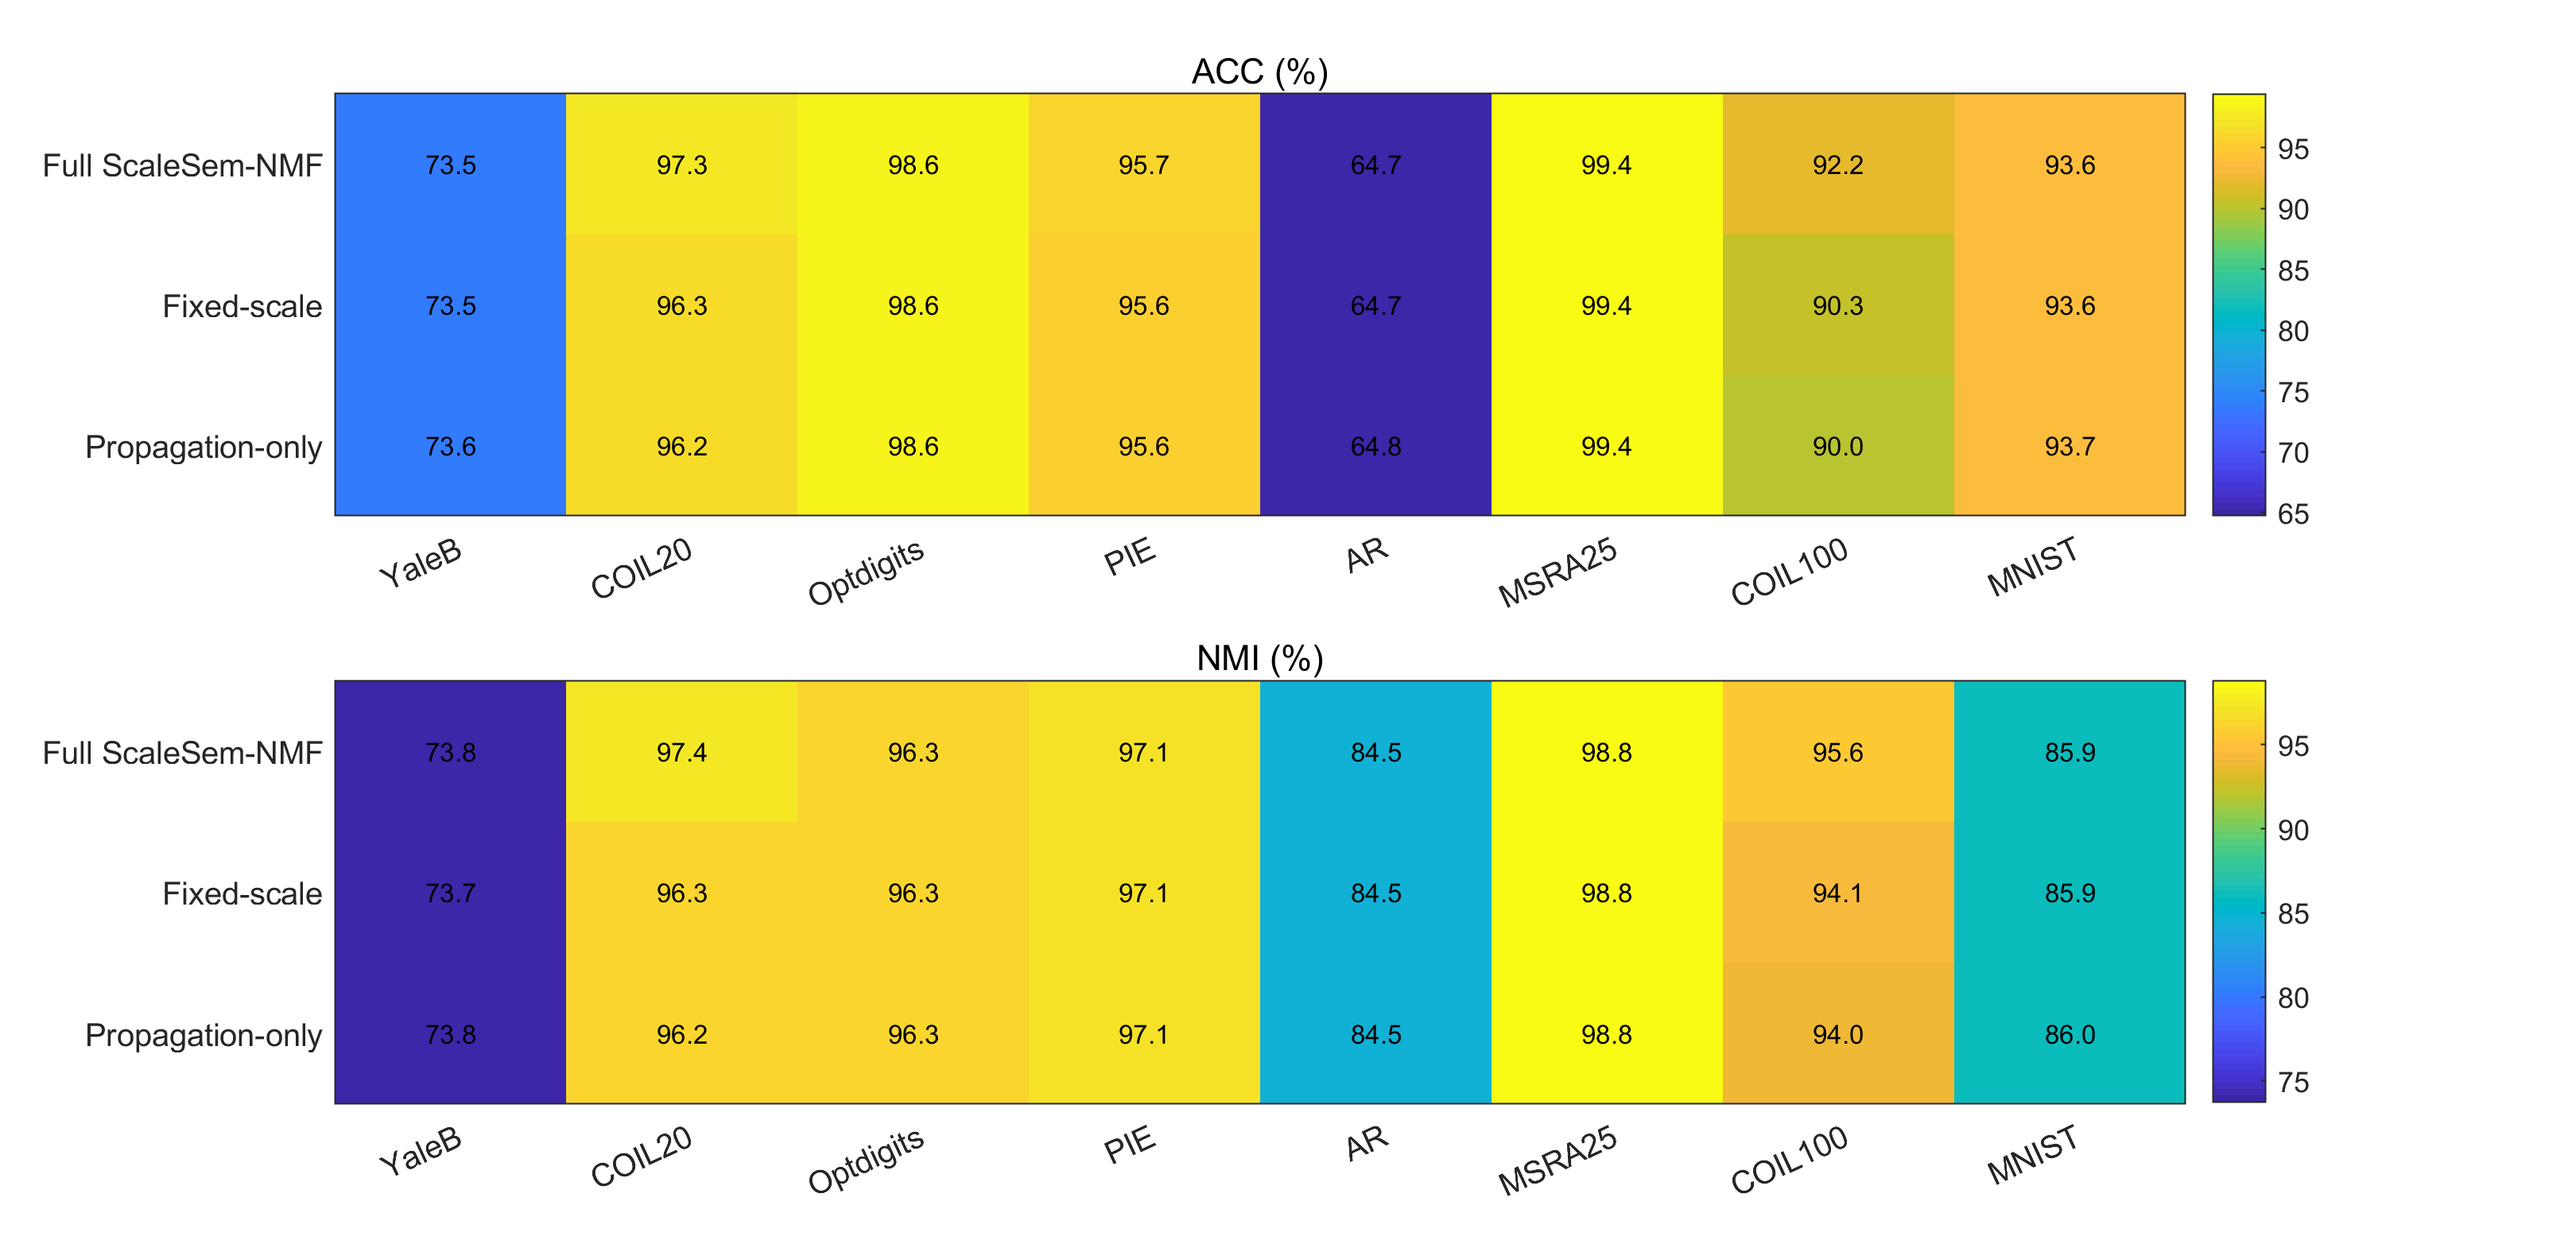
\includegraphics[width=0.90\textwidth,height=0.58\textheight,keepaspectratio]{figures/png/ablation-absolute-heatmap.png}
\caption{Mean absolute ACC and NMI over 20 paired seeds for the complete model and two controlled ablations. Absolute performance and paired differences answer complementary questions.}
\label{fig:ablation_heatmap}
\end{figure*}

\begin{figure*}[!htbp]
\centering
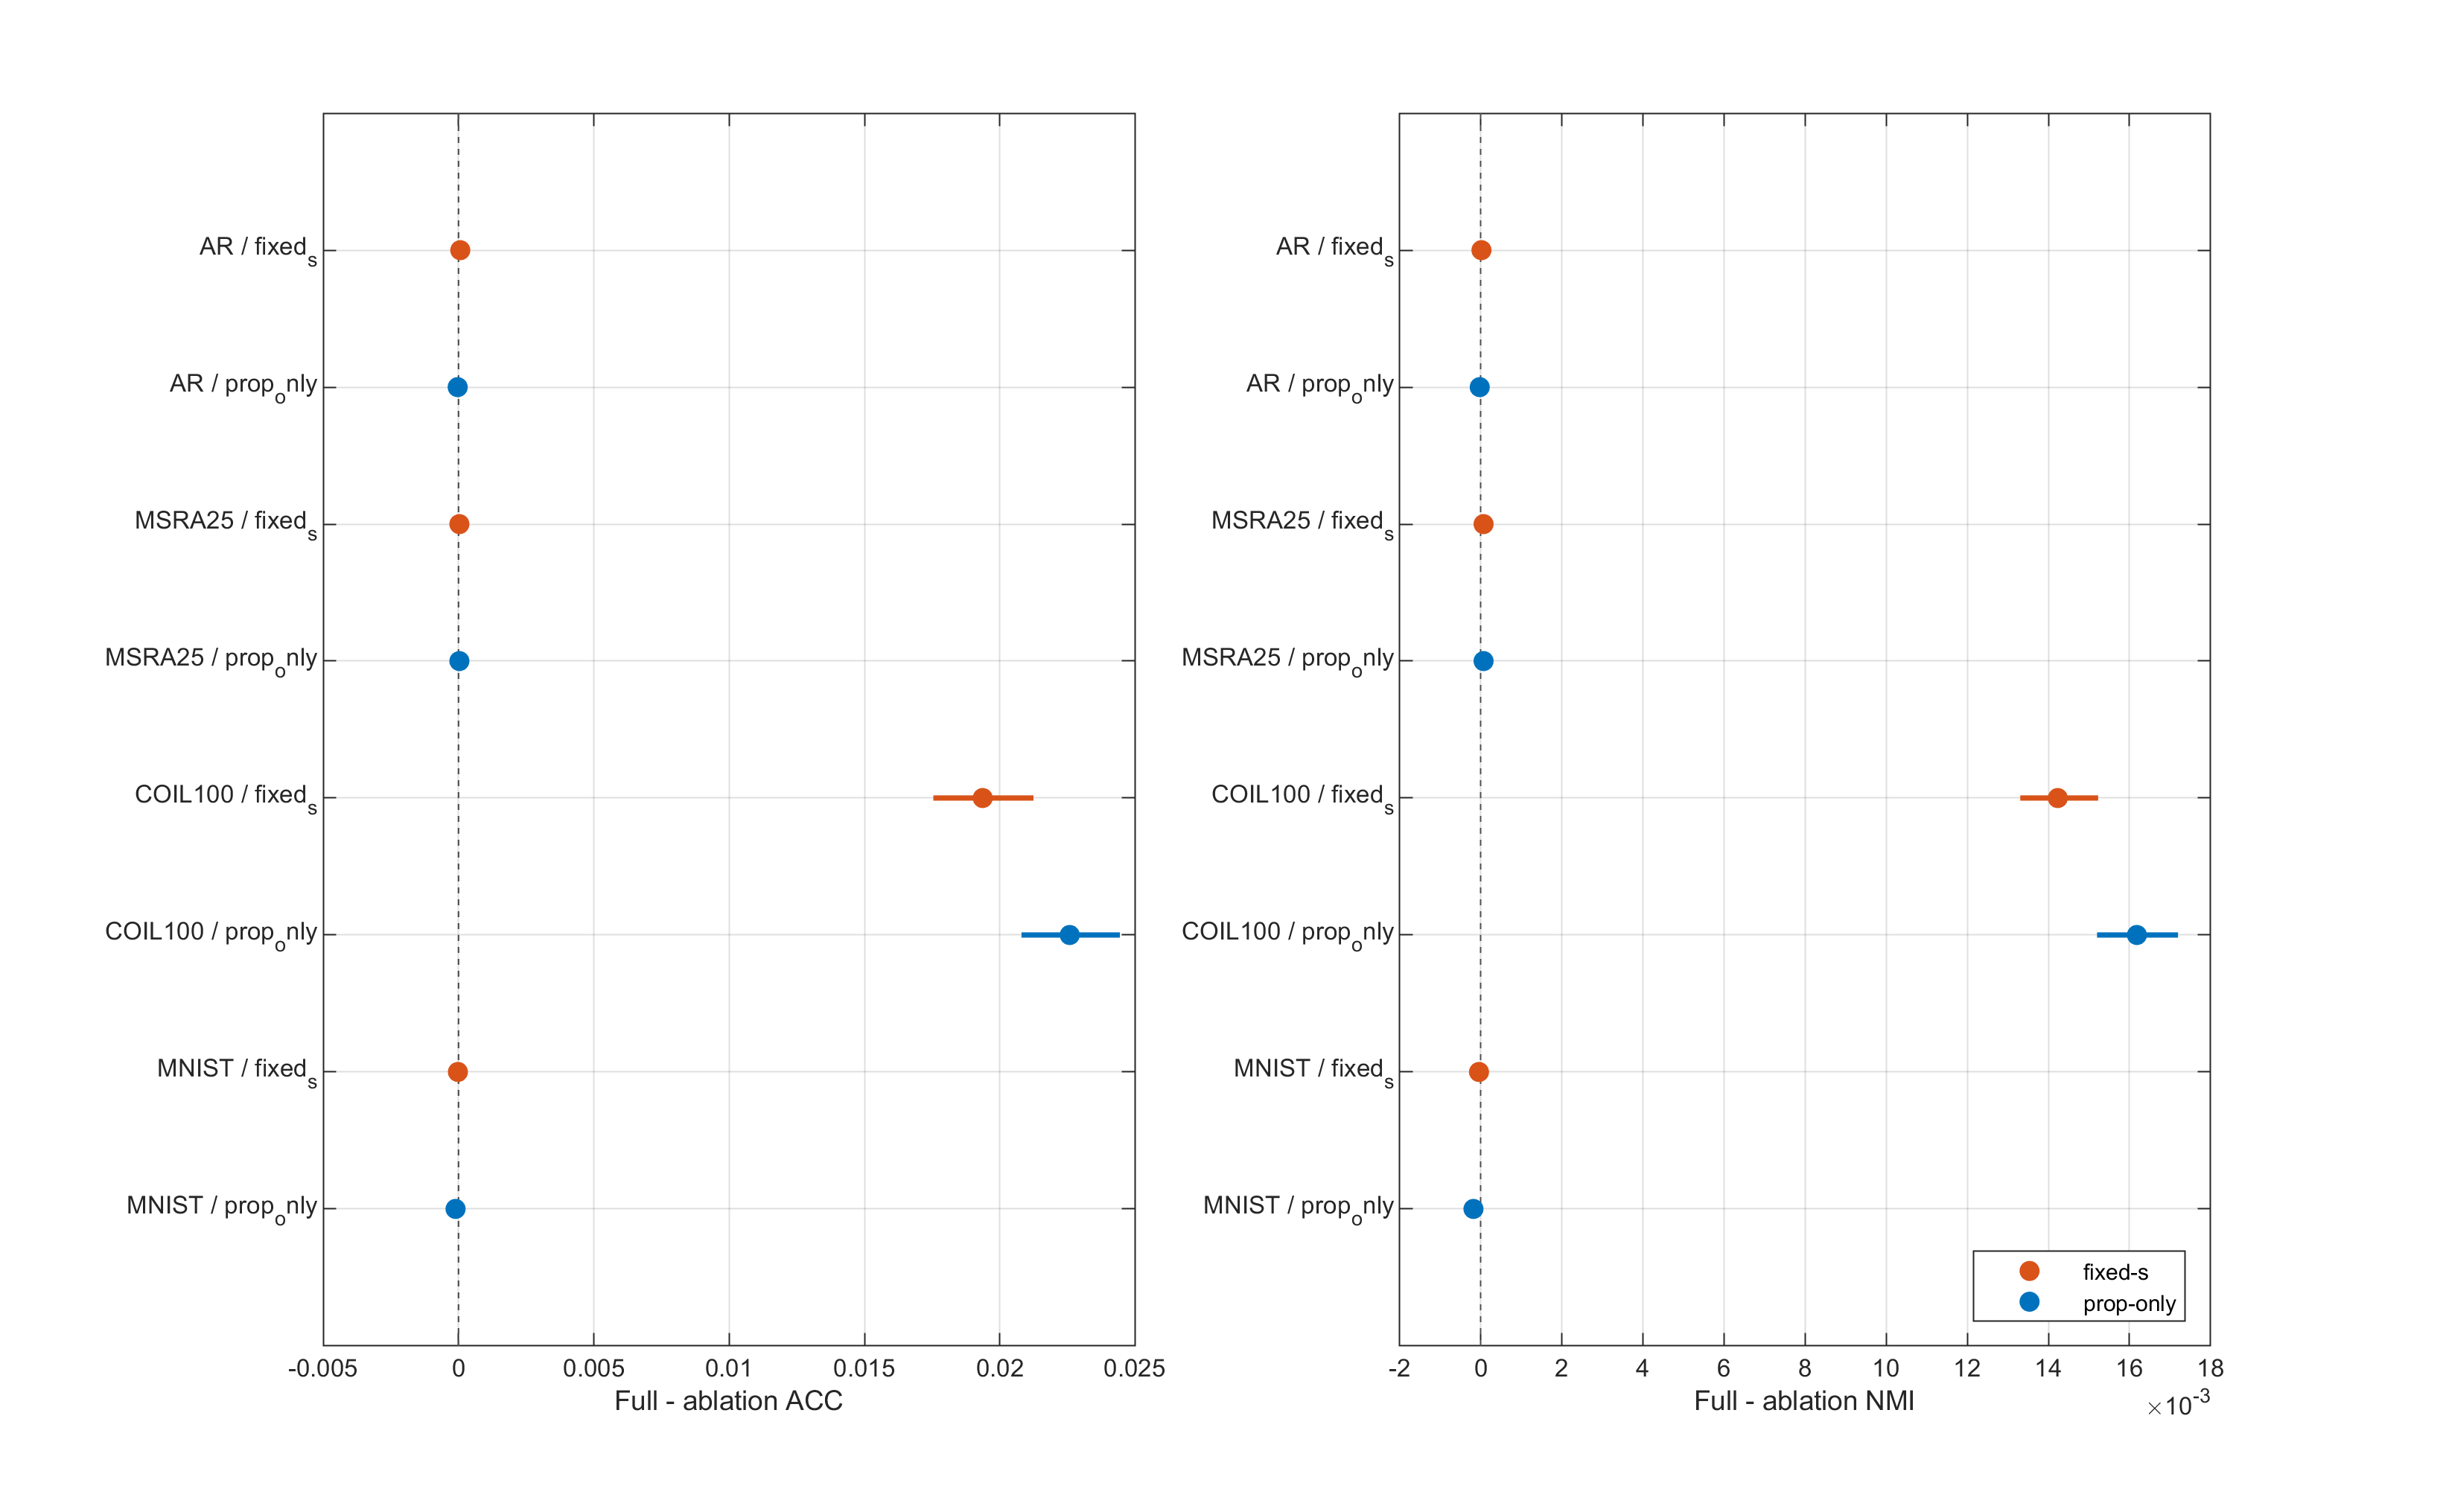
\includegraphics[width=0.84\textwidth,height=0.64\textheight,keepaspectratio]{figures/png/ablation-forest.png}
\caption{Controlled mechanism ablations with paired uncertainty intervals.}
\label{fig:ablation}
\end{figure*}

\FloatBarrier
\subsection{Cross-dataset mechanism diagnostics}

The ablation results identify where individual components help, but they do not by themselves explain why the effect varies across datasets. We therefore tested two preregistered explanatory hypotheses using only the existing 20-seed outputs on eight datasets, without retraining or parameter selection. The independent inferential unit is the dataset ($n=8$). First, we tested whether the dataset-level coefficient of variation of learned amplitudes is positively associated with the ACC and NMI benefit of adaptive scale over fixed scale. Second, we tested whether weaker alignment between reconstruction and propagation gradients is positively associated with the benefit of reconstruction coupling over propagation only. Exact one-sided Spearman permutation tests enumerate all $8!=40320$ dataset permutations, and leave-one-dataset-out analysis checks directional stability. Table~\ref{tab:regime} reports the exact tests and their leave-one-dataset-out directional checks.

\begin{table*}[!htbp]
\centering
\caption{Cross-dataset mechanism tests under the preregistered exact one-sided criterion. The table reports effect direction, exact probability, and leave-one-dataset-out stability.}
\label{tab:regime}
\scriptsize
\resizebox{\textwidth}{!}{%
\begin{tabular}{llrrr}
\toprule
Predictor & Ablation gain & Spearman $\rho$ & Exact $p$ & Minimum leave-one-out $\rho$ \\
\midrule
Scale CV & fixed-scale $\Delta$ACC & 0.5714 & 0.0756 & 0.5357 \\
Scale CV & fixed-scale $\Delta$NMI & 0.5476 & 0.0855 & 0.5000 \\
Negative gradient cosine & propagation-only $\Delta$ACC & 0.1905 & 0.3323 & 0.0357 \\
Negative gradient cosine & propagation-only $\Delta$NMI & 0.1905 & 0.3323 & 0.0357 \\
\bottomrule
\end{tabular}}
\end{table*}

Scale heterogeneity shows a positive but inconclusive association with adaptive-scale gains. The negative cosine is below zero for every dataset, indicating that the two raw gradients are aligned, with values closer to zero representing weaker alignment. The observed empirical benefits remain strongest on COIL20 and COIL100.

\FloatBarrier
\subsection{Convergence and implementation checks}

Across 20 seeds on each of eight datasets, all objective histories in Fig.~\ref{fig:convergence} are finite and no increase above tolerance is observed. YaleB, COIL20, PIE, and COIL100 reach the 200-iteration cap in every run and are reported as cap-limited. Optdigits, AR, MSRA25, and MNIST have median iteration counts 66, 98.5, 49.5, and 58. Independent finite-difference checks of the three analytical gradients have maximum relative errors \(9.20\times10^{-7}\), \(5.64\times10^{-7}\), and \(1.52\times10^{-6}\) for the \(U\), \(s\), and \(F\) blocks, respectively; simplex, label, nonnegativity, graph-symmetry, and gauge-normalization checks also pass. The numerical evidence establishes correct derivative implementation, feasible iterates, and finite monotone descent. Endpoint stationarity remains governed by the conditions of Theorem~2; the cap-limited runs are reported by their observed descent behavior.

\begin{figure*}[!htbp]
\centering
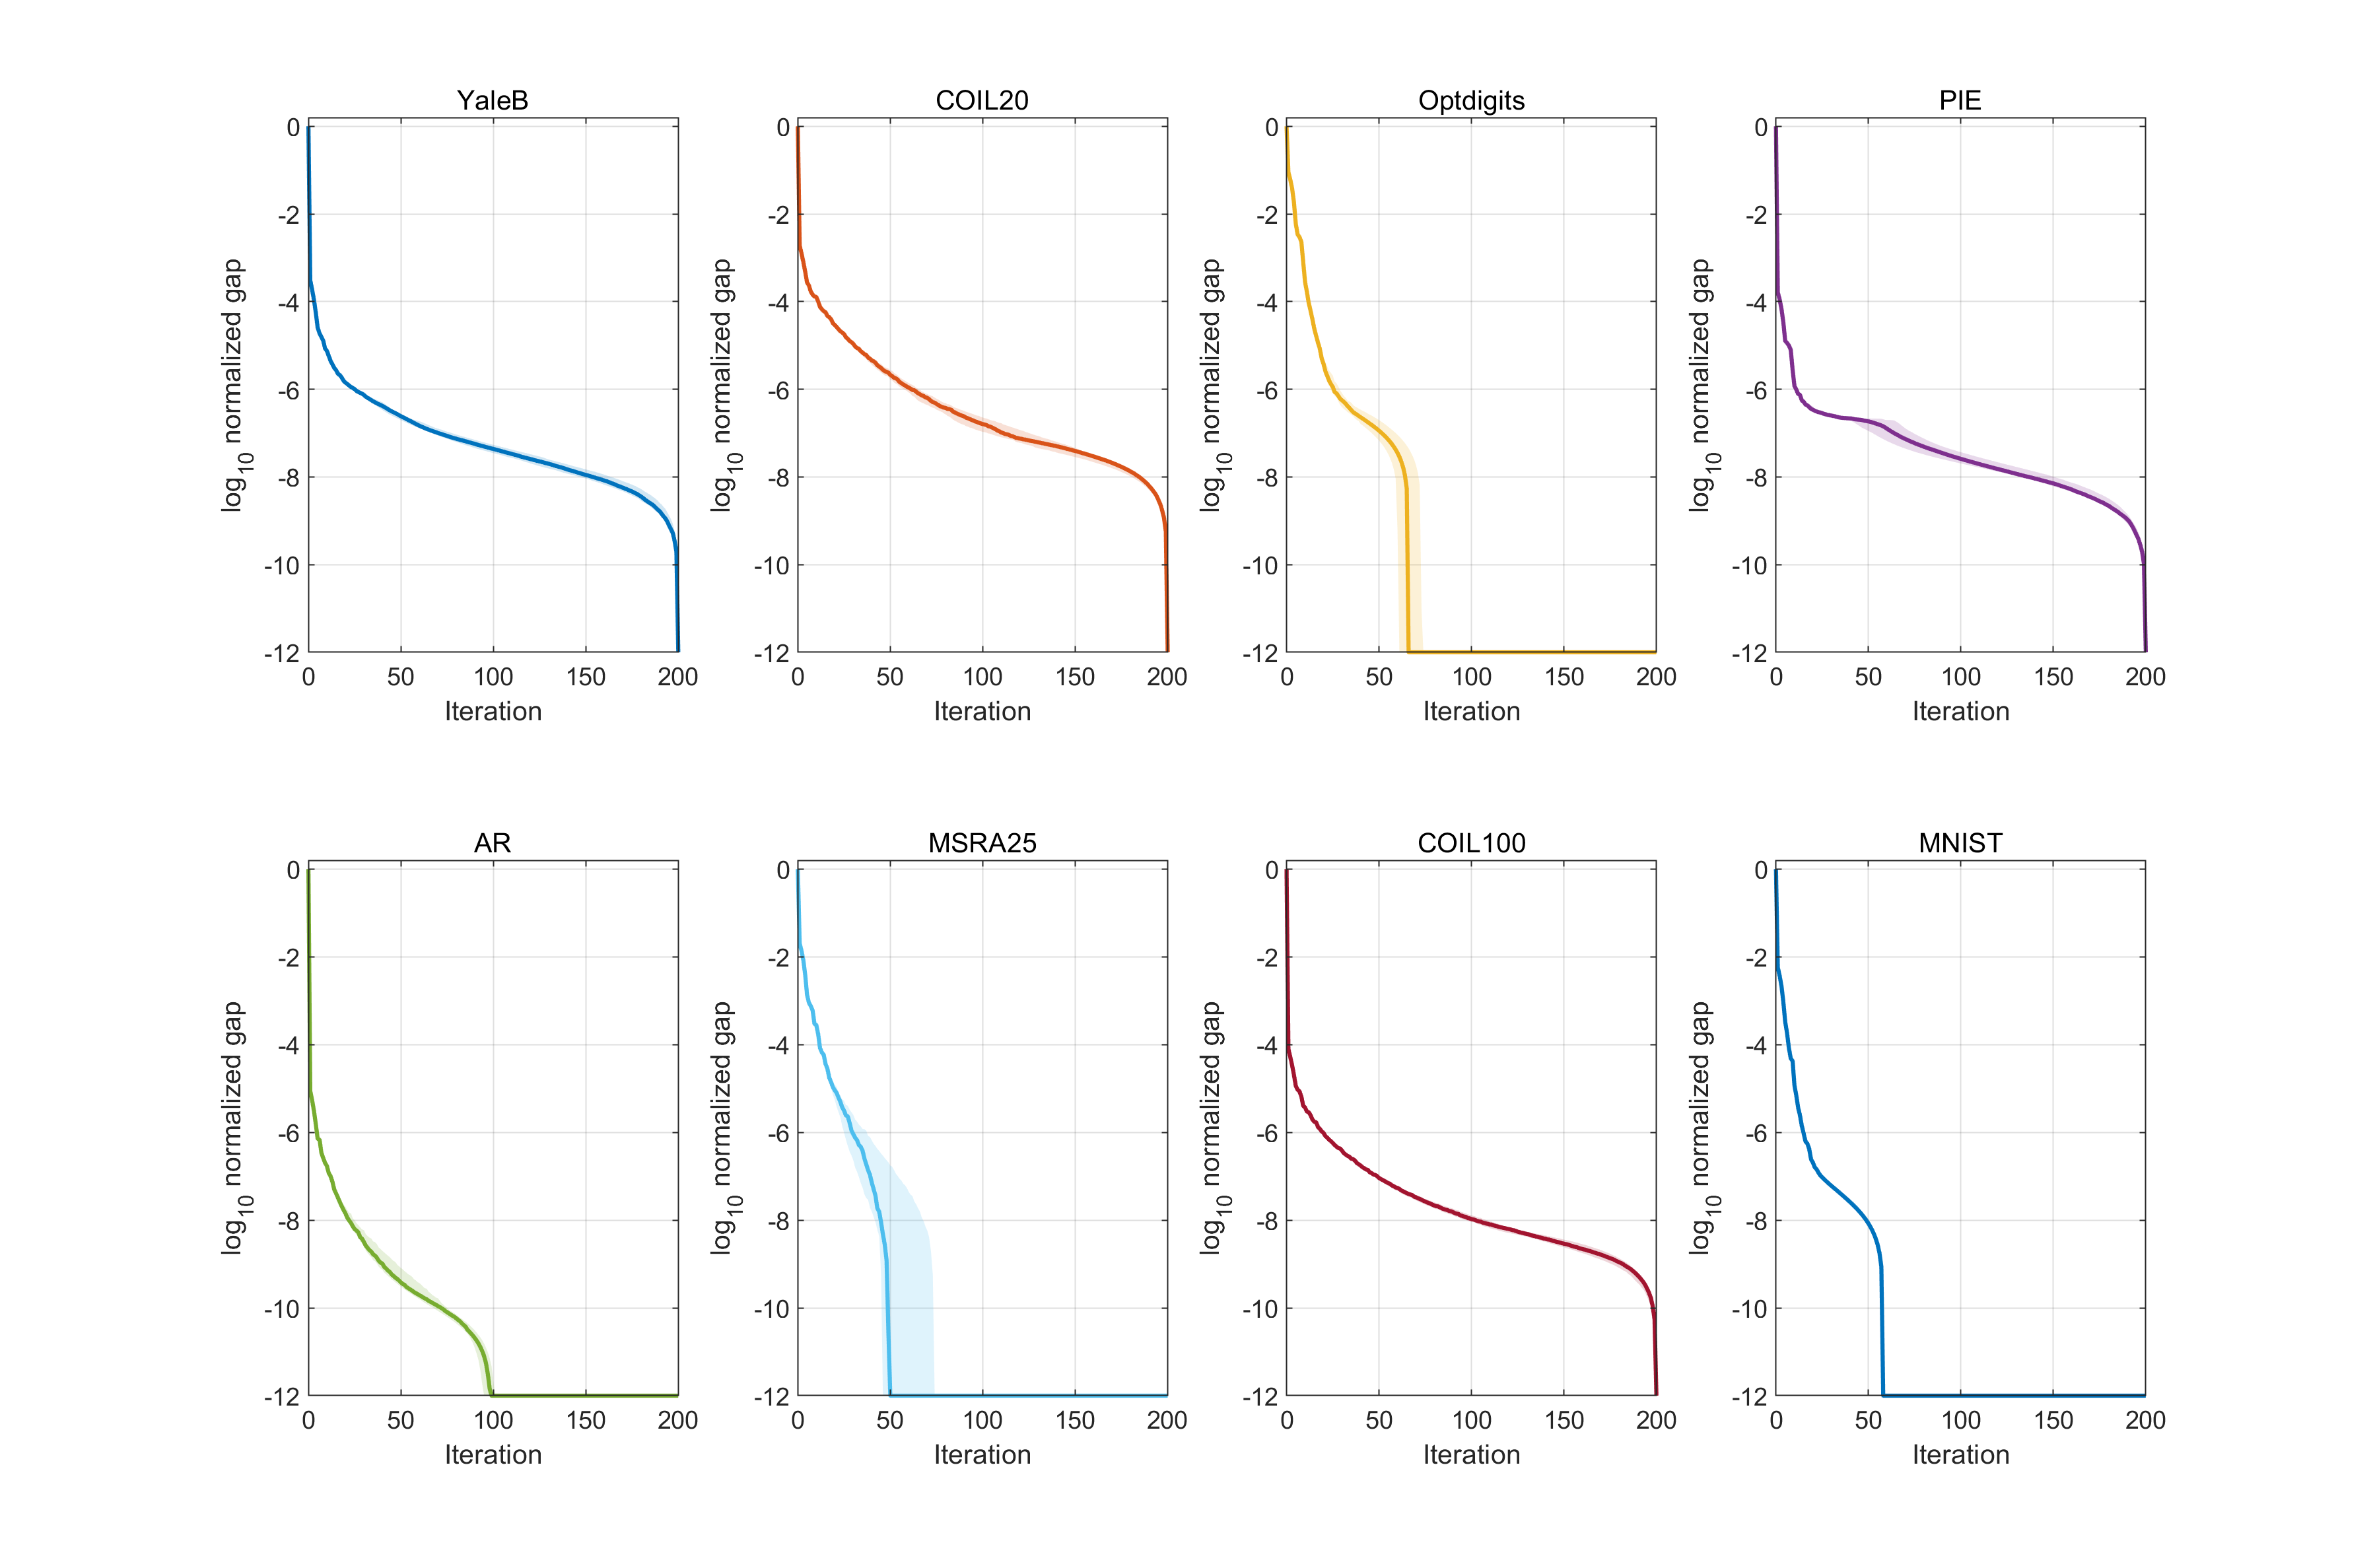
\includegraphics[width=0.88\textwidth,height=0.62\textheight,keepaspectratio]{figures/png/convergence.png}
\caption{Objective histories on eight datasets. The curves show finite monotone descent; the text identifies the runs that reach the iteration cap.}
\label{fig:convergence}
\end{figure*}

\FloatBarrier
\section{Discussion}

\subsection{Supported conclusion}

Scale-semantic separation is a coherent correction to point anchoring and produces meaningful empirical gains in identifiable regimes. COIL100 supplies the strongest evidence across baseline choice and statistical summary. COIL20 supplies strong evidence for the learned-amplitude mechanism. The supervision-budget and salt-and-pepper experiments extend this evidence beyond the clean 10\% protocol.

\subsection{Scope and computational profile}

The objective is nonconvex, and Theorem~2 states the regularity conditions for stationary accumulation points. Neighborhood size materially affects performance, and explicit high-order graph powers can become dense. Several datasets reach the iteration cap. Unified timing shows higher cost than GOCNMF and SNMFWLP across the tested datasets. The AR and selected external-baseline settings use preregistered domain-transfer parameters. The experimental scope covers the eight nonnegative datasets in Table~\ref{tab:datasets}.

\section{Conclusion}

ScaleSem-NMF decomposes every latent coefficient into a learned reconstruction amplitude and a simplex semantic direction, thereby preventing a one-hot label from fixing an arbitrary radial magnitude. The model is compact and directly decodable. Eight-dataset experiments identify clear success regimes on COIL20 and COIL100, stable gains on selected datasets, and practical parity elsewhere. Supervision-budget and salt-and-pepper experiments satisfy their preregistered criteria. Parameter and runtime experiments characterize neighborhood sensitivity and computational cost. Overall, ScaleSem-NMF provides an interpretable structural alternative for semi-supervised NMF.



\section*{CRediT authorship contribution statement}
\textit{Author-confirmed CRediT roles will be inserted in the submission version.}

\section*{Declaration of competing interest}
\textit{The competing-interest declaration will be inserted in the submission version.}

\section*{Funding}
\textit{The funding statement will be inserted in the submission version.}

\section*{Data and code availability}
The project archive contains the MATLAB R2019a implementation, frozen configuration files, paired labeled indices, random seeds, raw run-level metrics, and scripts used to generate every reported table and figure. YaleB, COIL20, PIE, AR, MSRA25, COIL100, and \texttt{MNIST\_Han.mat} follow the benchmark files distributed through the HLPNMF author package at \url{https://github.com/ljisxz/HLPNMF}; Optdigits uses the standard UCI benchmark version. Table~\ref{tab:datasets} summarizes the dataset dimensions, and Section~4.1 specifies the preprocessing protocol. Dataset files remain subject to their original distribution terms.

\begin{thebibliography}{99}
\bibitem{Jain1999Clustering} A. K. Jain, M. N. Murty, P. J. Flynn, Data clustering: A review, ACM Computing Surveys 31(3) (1999) 264--323. \doi{10.1145/331499.331504}.
\bibitem{Jain2010Clustering} A. K. Jain, Data clustering: 50 years beyond K-means, Pattern Recognition Letters 31(8) (2010) 651--666. \doi{10.1016/j.patrec.2009.09.011}.
\bibitem{VanEngelen2020Survey} J. E. van Engelen, H. H. Hoos, A survey on semi-supervised learning, Machine Learning 109(2) (2020) 373--440. \doi{10.1007/s10994-019-05855-6}.
\bibitem{Bair2013SSC} E. Bair, Semi-supervised clustering methods, WIREs Computational Statistics 5(5) (2013) 349--361. \doi{10.1002/wics.1270}.
\bibitem{Lee1999NMF} D. D. Lee, H. S. Seung, Learning the parts of objects by non-negative matrix factorization, Nature 401(6755) (1999) 788--791. \doi{10.1038/44565}.
\bibitem{Lee2001Algorithms} D. D. Lee, H. S. Seung, Algorithms for non-negative matrix factorization, in: Advances in Neural Information Processing Systems 13, 2001, pp. 556--562.
\bibitem{Gillis2014WhyHow} N. Gillis, The why and how of nonnegative matrix factorization, in: J. A. K. Suykens, M. Signoretto, A. Argyriou (Eds.), Regularization, Optimization, Kernels, and Support Vector Machines, Chapman and Hall/CRC, 2014, pp. 275--310. \doi{10.1201/b17558-15}.
\bibitem{Liu2012CNMF} H. Liu, Z. Wu, X. Li, D. Cai, T. S. Huang, Constrained nonnegative matrix factorization for image representation, IEEE Transactions on Pattern Analysis and Machine Intelligence 34(7) (2012) 1299--1311. \doi{10.1109/TPAMI.2011.217}.
\bibitem{Xing2021DSSNMF} Z. Xing, M. Wen, J. Peng, J. Feng, Discriminative semi-supervised non-negative matrix factorization for data clustering, Engineering Applications of Artificial Intelligence 103 (2021) 104289. \doi{10.1016/j.engappai.2021.104289}.
\bibitem{Li2025EDNMF} J. Li, X. Shen, C. Li, Y. Li, Elements discriminative non-negative matrix factorization for data clustering, Engineering Applications of Artificial Intelligence 156 (2025) 111210. \doi{10.1016/j.engappai.2025.111210}.
\bibitem{Shen2026LCNMF} X. Shen, J. Li, Locally constrained non-negative matrix factorization for data clustering, IEEE Access 14 (2026) 78907--78919. \doi{10.1109/ACCESS.2026.3696008}.
\bibitem{Cai2011GNMF} D. Cai, X. He, J. Han, T. S. Huang, Graph regularized nonnegative matrix factorization for data representation, IEEE Transactions on Pattern Analysis and Machine Intelligence 33(8) (2011) 1548--1560. \doi{10.1109/TPAMI.2010.231}.
\bibitem{Zeng2014HypergraphNMF} K. Zeng, J. Yu, C. Li, J. You, T. Jin, Image clustering by hypergraph regularized non-negative matrix factorization, Neurocomputing 138 (2014) 209--217.
\bibitem{Yi2015LpSNMF} Y. Yi, Y. Shi, H. Zhang, J. Wang, J. Kong, Label propagation based semi-supervised non-negative matrix factorization for feature extraction, Neurocomputing 149 (2015) 1021--1037. \doi{10.1016/j.neucom.2014.07.031}.
\bibitem{Lan2022LPNMF} L. Lan, T. Liu, X. Zhang, C. Xu, Z. Luo, Label propagated nonnegative matrix factorization for clustering, IEEE Transactions on Knowledge and Data Engineering 34(1) (2022) 340--351.
\bibitem{Wang2022PNLP} C. Wang, J. Zhang, T. Wu, M. Zhang, G. Shi, Semi-supervised nonnegative matrix factorization with positive and negative label propagations, Applied Intelligence 52(9) (2022) 9739--9750.
\bibitem{Li2025GOCNMF} J. Li, C. Li, Graph regularized one-hot-constrained nonnegative matrix factorization for data representation, Engineering Applications of Artificial Intelligence 156 (2025) 111224. \doi{10.1016/j.engappai.2025.111224}.
\bibitem{Li2025OCSNMF} J. Li, C. Li, One-hot constrained symmetric nonnegative matrix factorization for image clustering, Pattern Recognition 162 (2025) 111427.
\bibitem{Wang2015ConstraintNMF} D. Wang, X. Gao, X. Wang, Semi-supervised nonnegative matrix factorization via constraint propagation, IEEE Transactions on Cybernetics 46(1) (2016) 233--244.
\bibitem{Yin2023HSSNMF} J. Yin, S. Peng, Z. Yang, B. Chen, Z. Lin, Hypergraph based semi-supervised symmetric nonnegative matrix factorization for image clustering, Pattern Recognition 137 (2023) 109274.
\bibitem{Yang2025SPNMF} X. Yang, T. Zhu, S. Peng, F. Nie, Z. Lin, Semi-supervised pivotal-aware nonnegative matrix factorization with label and pairwise constraint propagation for data clustering, Pattern Recognition 157 (2025) 110933.
\bibitem{Mo2024PNLPSCNMF} Y. Mo, X. Li, J. Mei, Semi-supervised nonnegative matrix factorization with label propagation and constraint propagation, Engineering Applications of Artificial Intelligence 133 (2024) 108196.
\bibitem{Peng2021CSNMF} S. Peng, W. Ser, B. Chen, Z. Lin, Robust semi-supervised nonnegative matrix factorization for image clustering, Pattern Recognition 111 (2021) 107683. \doi{10.1016/j.patcog.2020.107683}.
\bibitem{Jing2025SNMFSP} W. Jing, L. Lu, W. Ou, Semi-supervised non-negative matrix factorization with structure preserving for image clustering, Neural Networks 187 (2025) 107340. \doi{10.1016/j.neunet.2025.107340}.
\bibitem{Jing2026SNMFWLP} W. Jing, L. Lu, W. Ou, Semi-supervised non-negative matrix factorization with weighted label propagation for data representation, Signal Processing 241 (2026) 110407. \doi{10.1016/j.sigpro.2025.110407}.
\bibitem{Li2026HLPNMF} J. Li, X. Zhou, X. Shen, C. Li, High-order label propagation-guided nonnegative matrix factorization for semi-supervised clustering, Pattern Recognition 180 (2026) 114657. \doi{10.1016/j.patcog.2026.114657}.
\bibitem{Chavoshinejad2023S4NMF} J. Chavoshinejad, S. A. Seyedi, F. Akhlaghian Tab, N. Salahian, Self-supervised semi-supervised nonnegative matrix factorization for data clustering, Pattern Recognition 137 (2023) 109282. \doi{10.1016/j.patcog.2022.109282}.
\bibitem{Zhu2003GaussianFields} X. Zhu, Z. Ghahramani, J. Lafferty, Semi-supervised learning using Gaussian fields and harmonic functions, in: Proceedings of the 20th International Conference on Machine Learning, 2003, pp. 912--919.
\bibitem{Zhou2004LGC} D. Zhou, O. Bousquet, T. N. Lal, J. Weston, B. Sch\"olkopf, Learning with local and global consistency, in: Advances in Neural Information Processing Systems 16, 2004.
\bibitem{Qiao2018GraphReview} L. Qiao, L. Zhang, S. Chen, D. Shen, Data-driven graph construction and graph learning: A review, Neurocomputing 312 (2018) 336--351.
\bibitem{Gao2022HypergraphReview} Y. Gao, Z. Zhang, H. Lin, X. Zhao, S. Du, C. Zou, Hypergraph learning: Methods and practices, IEEE Transactions on Pattern Analysis and Machine Intelligence 44(5) (2022) 2548--2566.
\bibitem{Song2023GSSLReview} Z. Song, X. Yang, Z. Xu, I. King, Graph-based semi-supervised learning: A comprehensive review, IEEE Transactions on Neural Networks and Learning Systems 34(11) (2023) 8174--8194.
\bibitem{Abdolali2021SSMF} M. Abdolali, N. Gillis, Simplex-structured matrix factorization: Sparsity-based identifiability and provably correct algorithms, SIAM Journal on Mathematics of Data Science 3(2) (2021) 593--623. \doi{10.1137/20M1354982}.
\bibitem{Abdolali2024DualSimplex} M. Abdolali, G. Barbarino, N. Gillis, Dual simplex volume maximization for simplex-structured matrix factorization, SIAM Journal on Imaging Sciences 17(4) (2024) 2362--2391. \doi{10.1137/24M1650600}.
\bibitem{Xing2021GNMFLD} Z. Xing, Y. Ma, X. Yang, F. Nie, Graph regularized nonnegative matrix factorization with label discrimination for data clustering, Neurocomputing 440 (2021) 297--309.
\bibitem{Kuhn1955Hungarian} H. W. Kuhn, The Hungarian method for the assignment problem, Naval Research Logistics Quarterly 2(1--2) (1955) 83--97.
\bibitem{Vinh2010NMI} N. X. Vinh, J. Epps, J. Bailey, Information theoretic measures for clusterings comparison: Is a correction for chance necessary?, Journal of Machine Learning Research 11 (2010) 2837--2854.
\bibitem{Wilcoxon1945} F. Wilcoxon, Individual comparisons by ranking methods, Biometrics Bulletin 1(6) (1945) 80--83.
\end{thebibliography}
\end{document}
